\chapter{高阶归纳类型 (Higher Inductive Types)}
\label{cha:hits}

\index{type!higher inductive|(}%
\indexsee{inductive!type!higher}{type, higher inductive}%
\indexsee{higher inductive type}{type, higher inductive}%

\section{引言 (Introduction)}
\label{sec:intro-hits}

\index{generation!of a type, inductive|(}

与我们在 \cref{cha:induction} 中讨论的一般归纳类型类似,高阶归纳类型 (higher inductive types) 是通过一些构造器生成新类型的一般模式。但与普通归纳类型不同,在定义高阶归纳类型时,我们可以有“构造器”不仅生成该类型的\emph{点},还生成该类型中的\emph{路径}和更高阶的路径。
\index{type!circle}%
\indexsee{circle type}{type,circle}%
例如,我们可以考虑由以下构造器生成的高阶归纳类型 $\Sn^1$:
\begin{itemize}
  \item 一个点 $\base:\Sn^1$,以及
  \item 一个路径 $\lloop : {\id[\Sn^1]\base\base}$。
\end{itemize}
这应当与例如 $\bool$ 的定义完全类似,$\bool$ 是由以下构造器生成的:
\begin{itemize}
  \item 一个点 $\bfalse:\bool$ 和
  \item 一个点 $\btrue:\bool$,
\end{itemize}
或由以下构造器生成的 $\nat$ 的定义:
\begin{itemize}
  \item 一个点 $0:\nat$ 以及
  \item 一个函数 $\suc:\nat\to\nat$。
\end{itemize}
当我们将类型视为高阶群体 (higher groupoids) 时,更一般的“生成”概念是非常自然的:由于高阶群体是一个具有路径和更高阶路径以及点的“多重排序对象”,我们应当允许所有维度上的“生成器”。

我们将普通类型的构造器(如 $\base$)称为\define{点构造器 (point constructors)}\indexdef{constructor!point}%
\indexdef{point!constructor}%
或\emph{普通构造器},而将其他构造器(如 $\lloop$)称为\define{路径构造器 (path constructors)}%
\indexdef{constructor!path}%
\indexdef{path!constructor}%
或\emph{高阶构造器}。每个路径构造器必须指定路径的起点和终点,我们称其为\define{源点 (source)}%
\indexdef{source!of a path constructor}%
和\define{目标 (target)};%
\indexdef{target!of a path constructor}%
对于 $\lloop$,源点和目标均为 $\base$。

请注意,路径构造器如 $\lloop$ 生成的是同一性类型 (identity type) 的一个\emph{新}元素,它(至少在\emph{先验}上)不等于任何先前存在的此类元素。特别地,$\lloop$ 先验上不等于 $\refl{\base}$(尽管证明它们确实不相等需要一些思考;见 \cref{thm:loop-nontrivial})。这就是 $\Sn^1$ 与普通归纳类型 \unit 的区别。

关于这种推广,有几个重要点需要说明。

\index{free!generation of an inductive type}%
首先,应认真对待“生成”一词,其意义与通过一些集合自由生成群相同。特别地,因为高阶群体带有路径和更高阶路径上的\emph{运算},当这种对象由某些构造器“生成”时,这些运算会创建更多不直接来自构造器的路径。例如,在高阶归纳类型 $\Sn^1$ 中,构造器 $\lloop$ 并不是唯一的从 $\base$ 到 $\base$ 的非平凡路径;我们还有“$\lloop\ct\lloop$”和“$\lloop\ct\lloop\ct\lloop$”等等,以及 $\opp{\lloop}$ 等,所有这些都是不同的。这可能看起来如此显而易见,以至于不值得一提,但它与“普通”归纳类型的行为有所不同,在“普通”归纳类型中,我们可以预期在归纳类型中看不到除直接由构造器“放入”的任何东西。

其次,这种生成确实是\emph{自由}生成的:高阶归纳类型实际上不允许我们施加“公理”,例如强制“$\lloop\ct\lloop$”等于 $\refl{\base}$。然而,在 $\infty$-群体%
\index{.infinity-groupoid@$\infty$-groupoid}
的世界中,“自由生成”和“表示”之间几乎没有区别,
\index{presentation!of an infinity-groupoid@of an $\infty$-groupoid}%
\index{generation!of an infinity-groupoid@of an $\infty$-groupoid}%
因为我们可以通过添加一个新的二维生成器将两个路径\emph{同伦地}等同(例如,在 $\base=\base$ 中的路径 $\lloop\ct\lloop = \refl{\base}$)。当然,我们需要担心这个新生成器是否应满足其自身的“公理”,等等,但原则上,任何“表示”都可以通过将公理转化为构造器而转换为“自由”表示。正如我们将看到的,通过添加“截断构造器 (truncation constructors)”我们可以使用高阶归纳类型来表达经典概念,例如群表示。

第三,尽管高阶归纳类型包含生成该类型\emph{路径}的“构造器”,它仍然是\emph{单一}类型的归纳定义。特别地,正如我们将看到的,它是具有普遍性质的高阶归纳类型本身(通常通过归纳原则表示),而\emph{不是}它的同一性类型。高阶归纳类型的同一性类型保留了任何同一性类型的通常归纳原则(即路径归纳),并未获得任何新的归纳原则。

因此,识别高阶归纳类型的同一性类型可能不是一件简单的事情,与我们在 \cref{cha:basics} 中能够给出显式描述所有传统类型构造操作下的同一性类型行为的方式形成对比。例如,$\Sn^1$ 中是否有从 $\base$ 到 $\base$ 的路径不是简单地由 $\lloop$ 及其逆元的副本复合而成的?直观上,答案应该是否定的(事实上也是),但证明这一点并不简单。实际上,这类问题迅速将我们引向诸如计算球体的同伦群这类问题,这是代数拓扑中一个长期存在的问题,并且没有已知的简单公式。同伦类型论为解决这些问题带来了新的强大视角,但它也要求类型论变得与这些问题的答案一样复杂。

\index{dimension!of path constructors}%
第四,构造器的“维度”(即它们输出点、路径、路径之间的路径等)与生成的类型在哪些维度上具有非平凡同伦之间没有直接联系。一个简单的例子是,如果一个归纳类型 $B$ 具有类型为 $A\to B$ 的构造器,那么 $A$ 中的任何路径和更高阶路径都会导致 $B$ 中的路径和更高阶路径,尽管该构造器根本不是“高阶”构造器。同样的事情也发生在高阶构造器中:具有类型 $A\to (\id[B]xy)$ 的构造器不仅意味着 $A$ 的点在 $B$ 中生成从 $x$ 到 $y$ 的路径,而且 $A$ 中的路径也会在这些路径之间生成路径,等等。正如我们将看到的,这种可能性是高阶归纳类型力量的主要来源之一。

另一方面,即使是不具有高阶类型输入的构造器也可能生成“意外”的高阶路径。例如,在由以下构造器生成的二维球体 $\Sn^2$ 中:
\symlabel{s2a}
\index{type!2-sphere}%
\begin{itemize}
  \item 一个点 $\base:\Sn^2$,以及
  \item 在 ${\base=\base}$ 中的二维路径 $\surf:\refl{\base} = \refl{\base}$,
\end{itemize}
存在一个从 $\refl{\refl{\base}}$ 到自身的非平凡\emph{三维路径}。拓扑学家会认识到这个路径是霍普夫纤维丛 (Hopf fibration) 的一个体现。从范畴论的角度来看,这与上面提到的 $\Sn^1$ 中包含的不仅仅是 $\lloop$ 还有 $\lloop\ct\lloop$ 等现象属于同一类:只不过在\emph{高阶}群体中,存在\emph{运算}能够提升维度。事实上,我们在 \cref{sec:equality} 中看到了许多这样的运算:结合律和单位律不仅仅是性质,而是运算,其输入是1路径,输出是2路径。

\index{generation!of a type, inductive|)}%

% In US Trade format it wants a page break here but then it stretches the above itemize,
% so we give it some stretchable space to use if it wants to.
\vspace*{0pt plus 20ex}

\section{归纳原则和依赖路径 (Induction principles and dependent paths)}
\label{sec:dependent-paths}

当我们描述像圆周这样的高阶归纳类型是由某些构造器生成时,我们必须通过给出类似于 \cref{cha:typetheory} 中基本类型构造器的规则来解释这意味着什么。构造器本身提供了\emph{引入规则},但要解释\emph{消去规则}(即归纳和递归原则)则需要更多思考。在本书中,我们不会尝试给出什么构成“高阶归纳定义”的一般表述以及如何从这种定义中提取消去规则——事实上,这是一个微妙的问题,当前正在研究中。相反,我们将依赖一些一般的非正式讨论和大量示例。

\index{type!circle}%
\index{recursion principle!for S1@for $\Sn^1$}%
递归原则通常很容易描述:给定任何带有与构造器为高阶归纳类型提供的结构相同的结构的类型,存在一个函数将构造器映射到该结构。例如,在 $\Sn^1$ 的情况下,递归原则表示给定一个带有点 $b:B$ 和路径 $\ell:b=b$ 的类型 $B$,存在一个函数 $f:\Sn^1\to B$ 使得 $f(\base)=b$ 且 $\apfunc f (\lloop) = \ell$。

\index{computation rule!for S1@for $\Sn^1$}%
\index{equality!definitional}%
然而,存在一个问题,即这些计算规则是判定性(judgmental)等式还是命题性等式(路径)。对于普通归纳类型,我们毫无顾虑地将其设为判定性等式,尽管我们在 \cref{cha:induction} 中看到,将它们设为命题性等式仍然会产生同一类型(等同于等价关系)。在普通情况下,可以认为计算规则实际上是\emph{定义性}等式,如导言中描述的直观意义那样。

\index{equality!judgmental}%
对于高阶归纳类型,这一点就不那么清楚了。%
更重要的是,由于运算 $\apfunc f$ 并不是真正的类型论的基本部分,而是我们使用同一性类型的归纳原则\emph{定义}的东西(我们也可以用其他等价的方式定义),因此在\emph{判定性}等式中显式引用它似乎不合适。判定性等式是推理系统的一部分,不应依赖我们可能在该系统\emph{内部}做出的特定定义选择。还有语义和实现问题需要考虑;参见注释。

将高阶归纳类型的\emph{点}构造器的计算规则设为判定性似乎是无问题的。在上面的例子中,这意味着我们有 $f(\base)\jdeq b$,判定性地。这种选择促进了高阶归纳类型的计算视角。而且,这也极大地简化了我们的工作,否则第二个计算规则 $\apfunc f (\lloop) = \ell$ 作为命题性等式将无法良好定义;我们将不得不将其一侧或另一侧与 $f(\base)$ 和 $b$ 的指定同一性进行复合。(当然,当我们谈论更高维度的路径时,这种问题确实会出现,但在这里这不会是我们关心的重点。另见 \cref{sec:hubs-spokes}。)因此,我们将点构造器的计算规则视为判定性,而路径和更高阶路径的计算规则视为命题性。%
\footnote{特别地,在 \cref{sec:types-vs-sets} 的语言中,这意味着我们的高阶归纳类型是\emph{规则}(规定如何引入这些类型及其元素、其归纳原则以及其点构造器的计算规则)和\emph{公理}(路径构造器的计算规则,断言某些同一性类型由未指定的项占据)的混合体。我们可以希望最终会有一个更好的类型论,其中高阶归纳类型像同值性 (univalence) 一样,仅使用规则而没有公理。%
\indexfoot{axiom!versus rules}%
\indexfoot{rule!versus axioms}%
}

\begin{rmk}\label{rmk:defid}
回想一下,对于普通归纳类型,我们将递归定义函数的计算规则视为不仅仅是判定性等式,而是\emph{定义性}等式,因此我们可以使用 $\defeq$ 符号。例如,截断前驱函数 (truncated predecessor) $p:\nat\to\nat$ 定义为 $p(0)\defeq 0$ 和 $p(\suc(n))\defeq n$。在高阶归纳类型的情况下,这种符号对于点构造器(例如 $f(\base)\defeq b$)是合理的,但对于路径构造器可能会产生误导,因为等式 $\ap f \lloop = \ell$ 并不是判定性的。因此,我们混合使用符号,而是写成 $\ap f \lloop \defid \ell$ 表示这种“定义上的命题性等式”。
\end{rmk}
\index{computation rule!for higher inductive types|)}%
\index{computation rule!propositional|)}%

\index{type!circle|(}%
\index{induction principle!for S1@for $\Sn^1$}%
现在,归纳原则(依赖消去)又如何呢?回想一下,对于一个普通归纳类型 $W$,要通过归纳证明 $\prd{x:W} P(x)$,我们必须为 $W$ 的每个构造器指定一个作用于 $P$ 的运算,该运算作用于 $W$ 中该构造器之上的“纤维”。例如,如果 $W$ 是自然数 $\nat$,那么要通过归纳证明 $\prd{x:\nat} P(x)$,我们必须指定
\begin{itemize}
  \item 一个在构造器 $0:\nat$ 之上的纤维中的元素 $b:P(0)$,以及
  \item 对于每个 $n:\nat$,一个函数 $P(n) \to P(\suc(n))$。
\end{itemize}
第二个可以被视为一个位于构造器 $\suc:\nat\to\nat$ 之上的“$P\to P$”函数,一般化为 $b:P(0)$ 位于构造器 $0:\nat$ 之上。

类比地,要证明 $\prd{x:\Sn^1} P(x)$,我们应当指定
\begin{itemize}
  \item 一个在构造器 $\base:\Sn^1$ 之上的纤维中的元素 $b:P(\base)$,以及
  \item 一个从 $b$ 到 $b$ 的路径“位于构造器 $\lloop:\base=\base$ 之上”。
\end{itemize}
请注意,尽管 $\Sn^1$ 包含 $\lloop$ 以外的路径(如 $\refl{\base}$ 和 $\lloop\ct\lloop$),我们只需要指定一个位于构造器\emph{本身}之上的路径。这表达了 $\Sn^1$ 是“由其构造器自由生成”的直觉。

然而,问题是,从 $b$ 到 $b$ 的路径“位于”另一条路径之上是什么意思。这绝对不意味着仅仅是一条 $b=b$ 的路径,因为那将是一条位于纤维 $P(\base)$ 中的路径(在拓扑上,位于 $\base$ 处的\emph{恒等}路径之上的路径)。然而,实际上,我们已经在 \cref{cha:basics} 中回答了这个问题:在 \cref{lem:mapdep} 之前的讨论中,我们得出结论,从 $u:P(x)$ 到 $v:P(y)$ 的一条路径位于 $p:x=y$ 之上可以用纤维 $P(y)$ 中的路径 $\trans p u = v$ 表示。由于在本章中我们将大量使用这种\define{依赖路径}%
\index{path!dependent}%
,因此我们为它们引入一个特殊符号:
\begin{equation}
(\dpath P p u v) \defeq (\transfib{P} p u = v).\label{eq:dpath}
\end{equation}

\begin{rmk}
  定义依赖路径还有其他可能的方法。例如,我们可以考虑 $u = \trans{(\opp p)}{v}$,而不是 $\trans p u = v$。我们还可以将其作为更一般的“异质等式 (heterogeneous equality)”的特例获得,
  \index{heterogeneous equality}%
  \index{equality!heterogeneous}%
  或直接定义为归纳类型族。所有这些定义都会导致等价类型,因此从这个意义上讲,我们选择哪一个并不重要。然而,选择 $\trans p u = v$ 作为定义使得推导依赖路径的其他内容变得最容易,例如 $\apdfunc{f}$ 生成它们的方式,或我们可以使用 \cref{sec:computational} 中的传递引理 (transport lemmas) 在特定类型族中计算它们。
\end{rmk}

有了依赖路径的概念,我们现在可以更精确地陈述 $\Sn^1$ 的归纳原则:给定 $P:\Sn^1\to\type$ 和
\begin{itemize}
  \item 一个元素 $b:P(\base)$,以及
  \item 一个路径 $\ell : \dpath P \lloop b b$,
\end{itemize}
存在一个函数 $f:\prd{x:\Sn^1} P(x)$,使得 $f(\base)\jdeq b$ 并且 $\apd f \lloop = \ell$。与非依赖情况类似,我们称通过 $f(\base)\defeq b$ 和 $\apd f \lloop \defid \ell$ 定义 $f$。

\begin{rmk}\label{rmk:varies-along}
在非正式描述此归纳原则的应用时,我们将其视为将目标“$P(x)$ 对于所有 $x:\Sn^1$”分为两种情况,有时我们会使用诸如“当 $x$ 是 $\base$ 时”和“当 $x$ 沿 $\lloop$ 变化时”之类的短语引入这两个部分。%
\index{vary along a path constructor}%
这里没有为“沿路径变化”指定具体的数学含义:这只是表示相应证明部分的开始的一种方便方式;参见 \cref{thm:S1-autohtpy} 了解示例。
\end{rmk}

拓扑上,$\Sn^1$ 的归纳原则可以如 \cref{fig:topS1ind} 所示进行可视化。给定一个圆周上的纤维丛(在图中是一个环面),定义此纤维丛的截面等同于给出一个 $\base$ 上的纤维中的点 $b$ 以及一个从 $b$ 到 $b$ 位于 $\lloop$ 之上的路径。我们从类型论的角度理解这一点,使用我们的依赖路径定义,如 \cref{fig:ttS1ind} 所示:从 $b$ 到 $b$ 沿 $\lloop$ 的路径在纤维 $P(\base)$ 中由 $\trans \lloop b$ 到 $b$ 的路径表示。

\begin{figure}
  \centering
  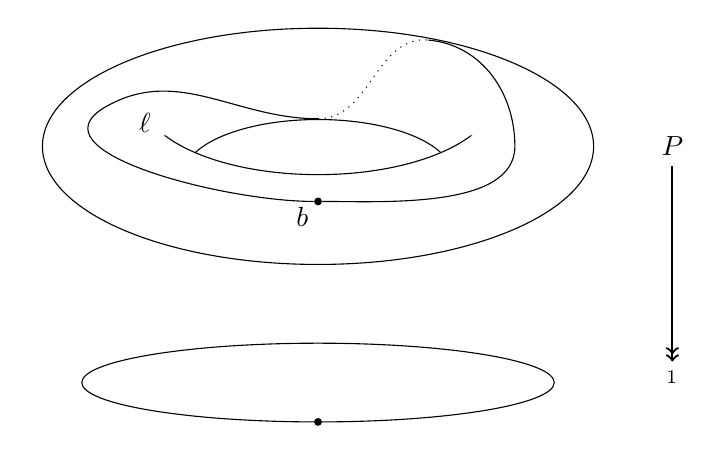
\begin{tikzpicture}
    \draw (0,0) ellipse (3 and .5);
    \draw (0,3) ellipse (3.5 and 1.5);
    \begin{scope}[yshift=4]
      \clip (-3,3) -- (-1.8,3) -- (-1.8,3.7) -- (1.8,3.7) -- (1.8,3) -- (3,3) -- (3,0) -- (-3,0) -- cycle;
      \draw[clip] (0,3.5) ellipse (2.25 and 1);
      \draw (0,2.5) ellipse (1.7 and .7);
    \end{scope}
    \node (P) at (4.5,3) {$P$};
    \node (S1) at (4.5,0) {$\Sn^1$};
    \draw[->>,thick] (P) -- (S1);
    \node[fill,circle,inner sep=1pt,label={below right:$\base$}] at (0,-.5) {};
    \node at (-2.6,.6) {$\lloop$};
    \node[fill,circle,\OPTblue,inner sep=1pt] (b) at (0,2.3) {};
    \node[\OPTblue] at (-.2,2.1) {$b$};
    \begin{scope}
      \draw[\OPTblue] (b) to[out=180,in=-150] (-2.7,3.5) to[out=30,in=180] (0,3.35);
      \draw[\OPTblue,dotted] (0,3.35) to[out=0,in=175] (1.4,4.35);
      \draw[\OPTblue] (1.4,4.35) to[out=-5,in=90] (2.5,3) to[out=-90,in=0,looseness=.8] (b);
    \end{scope}
    \node[\OPTblue] at (-2.2, 3.3) {$\ell$};
  \end{tikzpicture}
  \caption{圆周 $\Sn^1$ 的拓扑归纳原则}
  \label{fig:topS1ind}
\end{figure}

\begin{figure}
  \centering
  \begin{tikzpicture}
    \draw (0,0) ellipse (3 and .5);
    \draw (0,3) ellipse (3.5 and 1.5);
    \begin{scope}[yshift=4]
      \clip (-3,3) -- (-1.8,3) -- (-1.8,3.7) -- (1.8,3.7) -- (1.8,3) -- (3,3) -- (3,0) -- (-3,0) -- cycle;
      \draw[clip] (0,3.5) ellipse (2.25 and 1);
      \draw (0,2.5) ellipse (1.7 and .7);
    \end{scope}
    \node (P) at (4.5,3) {$P$};
    \node (S1) at (4.5,0) {$\Sn^1$};
    \draw[->>,thick] (P) -- (S1);
    \node[fill,circle,inner sep=1pt,label={below right:$\base$}] at (0,-.5) {};
    \node at (-2.6,.6) {$\lloop$};
    \node[fill,circle,\OPTblue,inner sep=1pt] (b) at (0,2.3) {};
    \node[\OPTblue] at (-.3,2.3) {$b$};
    \node[fill,circle,\OPTpurple,inner sep=1pt] (tb) at (0,1.8) {};
    % \draw[\OPTpurple,dashed] (b) to[out=0,in=0,looseness=5] (0,4) to[out=180,in=180] (tb);
    \draw[\OPTpurple,dashed] (b) arc (-90:90:2.9 and 0.85) arc (90:270:2.8 and 1.1);
    \begin{scope}
      \clip (b) -- ++(.1,0) -- (.1,1.8) -- ++(-.2,0) -- ++(0,-1) -- ++(3,2) -- ++(-3,0) -- (-.1,2.3) -- cycle;
      \draw[\OPTred,dotted,thick] (.2,2.07) ellipse (.2 and .57);
      \begin{scope}
        % \draw[clip] (b) -- ++(.1,0) |- (tb) -- ++(-.2,0) -- ++(0,-1) -| ++(3,3) -| (b);
        \clip (.2,0) rectangle (-2,3);
        \draw[\OPTred,thick] (.2,2.07) ellipse (.2 and .57);
      \end{scope}
    \end{scope}
    \node[\OPTred] at (1,1.2) {$\ell: \trans \lloop b=b$};
  \end{tikzpicture}
  \caption{圆周 $\Sn^1$ 的类型论归纳原则}
  \label{fig:ttS1ind}
\end{figure}

当然,我们期望可以通过将 $P$ 设为常类型族来从归纳原则推导出递归原则。事实上确实如此,尽管从依赖的 $\lloop$ 计算规则(它涉及 $\apdfunc f$)推导出非依赖的计算规则(它涉及 $\apfunc f$)出人意料地有点棘手。

\begin{lem}\label{thm:S1rec}
\index{递归原则!for S1@for $\Sn^1$}%
\index{计算规则!for S1@for $\Sn^1$}%
如果 $A$ 是一个带有 $a:A$ 和 $p:\id[A]aa$ 的类型,那么存在一个
函数 $f:\Sn^1\to{}A$ 使得
\begin{align*}
  f(\base)&\defeq a \\
  \apfunc f(\lloop)&\defid p.
\end{align*}
\end{lem}
\begin{proof}
  我们想要将 $\Sn^1$ 的归纳原则应用于常类型族 $(\lam{x} A): \Sn^1\to \UU$。为此所需的假设是 $(\lam{x} A)(\base) \jdeq A$ 的一点,我们有(即 $a:A$),以及 $\dpath {x \mapsto A}{\lloop} a a$ 中的一个依赖路径,或等价地 $\transfib{x \mapsto A}{\lloop} a = a$。该类型与 $p$ 所在的类型 $\id[A]aa$ 不同,但它等价于后者,因为根据 \cref{thm:trans-trivial} 我们有 $\transconst{A}{\lloop}{a} : \transfib{x \mapsto A}{\lloop} a= a$。因此,给定 $a:A$ 和 $p:a=a$,我们可以考虑复合
  \[\transconst{A}{\lloop}{a} \ct p:(\dpath {x \mapsto A}\lloop aa)。\]
  应用归纳原则,我们得到 $f:\Sn^1\to A$ 使得
  \begin{align}
    f(\base) &\jdeq a \qquad\text{and}\label{eq:S1recindbase}\\
    \apdfunc f(\lloop) &= \transconst{A}{\lloop}{a} \ct p。\label{eq:S1recindloop}
  \end{align}
  现在需要推导出 $\apfunc f(\lloop)=p$ 等式。然而,根据 \cref{thm:apd-const},我们有
  \[\apdfunc f(\lloop) = \transconst{A}{\lloop}{f(\base)} \ct \apfunc f(\lloop)。\]
  将此与~\eqref{eq:S1recindloop} 结合,并取消 $\transconstf$ 的出现(根据~\eqref{eq:S1recindbase} 它们是相同的),我们得到 $\apfunc f(\lloop)=p$。
\end{proof}

% 同样,在这种情况下,我们将通过 $f(\base)\defeq a$ 和 $\ap f \lloop \defid p$ 定义的 $f$ 视为定义。
我们还有一个相应的唯一性原则。

\begin{lem}\label{thm:uniqueness-for-functions-on-S1}
\index{唯一性!原则,命题性!对于圆周上的函数}%
如果 $A$ 是一个类型,且 $f,g:\Sn^1\to{}A$ 是两个映射,$p,q$ 是两个
等式:
\begin{align*}
  p:f(\base)&=_Ag(\base),\\
  q:\map{f}\lloop&=^{\lam{x} x=_Ax}_p\map{g}\lloop。
\end{align*}
那么对于所有 $x:\Sn^1$,我们有 $f(x)=g(x)$。
\end{lem}
\begin{proof}
  我们在类型族 $P(x)\defeq(f(x)=g(x))$ 处应用 $\Sn^1$ 的归纳原则。当 $x$ 为 $\base$ 时,$p$ 正是我们需要的。当 $x$ 沿 $\lloop$ 变化时,我们需要
  \(p=^{\lam{x} f(x)=g(x)}_{\lloop} p,\)
  根据 \cref{thm:transport-path,thm:dpath-path} 这一点可以简化为 $q$。
\end{proof}

\index{universal!property!of S1@of $\Sn^1$}%
这两个引理暗示了圆周的预期普遍性质:

\begin{lem}\label{thm:S1ump}
对于任何类型 $A$,我们有一个自然的等价
\[ (\Sn^1 \to A) \;\eqvsym\;
\sm{x:A} (x=x)。
\]
\end{lem}
\begin{proof}
  我们有一个标准函数 $f:(\Sn^1 \to A) \to \sm{x:A} (x=x)$,定义为 $f(g) \defeq (g(\base),\ap g \lloop)$。反过来,我们有 $g:\sm{x:A} (x=x) \to (\Sn^1 \to A)$,定义为将一对 $(b,\ell)$ 变为由圆周的递归原则给出的函数 $\Sn^1 \to A$。

  现在,通过圆周递归原则的计算规则,$f \circ g \htpy \idfunc$。而且通过唯一性原则,由于\((g \circ f)(\lloop) =^{\lam{x} x=_Ax}_{\refl{\base}} \lloop\),再加上圆周递归原则的计算规则,$g \circ f \htpy \idfunc$。因此,$f$ 有一个准逆元 (quasi-inverse),因此是一个等价。
\end{proof}

\index{type!circle|)}%

与 \cref{sec:htpy-inductive} 中一样,我们可以表明 \cref{thm:S1ump} 的结论等价于具有命题性计算规则的归纳原则。其他高阶归纳类型也满足类似于 \cref{thm:S1rec,thm:S1ump} 的引理;我们通常会将它们的证明留给读者。现在我们继续考虑许多示例。

\section{区间 (The interval)}
\label{sec:interval}

\index{类型!区间|(defstyle}%
\indexsee{区间!类型}{type, interval}%
\define{区间 (interval)},我们记作 $\interval$,它可能比圆更简单的高阶归纳类型。
它由以下部分生成:
\begin{itemize}
  \item 一个点 $\izero:\interval$,
  \item 一个点 $\ione:\interval$, 和
  \item 一条路径 $\seg : \id[\interval]\izero\ione$.
\end{itemize}
\index{递归原理!区间类型}%
区间的递归原理表明,给定一个类型 $B$ 以及
\begin{itemize}
  \item 一个点 $b_0:B$,
  \item 一个点 $b_1:B$, 和
  \item 一条路径 $s:b_0=b_1$,
\end{itemize}
存在一个函数 $f:\interval\to B$ 使得 $f(\izero)\jdeq b_0$, $f(\ione)\jdeq b_1$, 并且 $\ap f \seg = s$。
\index{归纳原理!区间类型}%
归纳原理表明,给定 $P:\interval\to\type$ 以及
\begin{itemize}
  \item 一个点 $b_0:P(\izero)$,
  \item 一个点 $b_1:P(\ione)$, 和
  \item 一条路径 $s:\dpath{P}{\seg}{b_0}{b_1}$,
\end{itemize}
存在一个函数 $f:\prd{x:\interval} P(x)$ 使得 $f(\izero)\jdeq b_0$, $f(\ione)\jdeq b_1$, 并且 $\apd f \seg = s$。

纯粹从同伦角度来看,区间并不是真的有趣:

\begin{lem}\label{thm:contr-interval}
类型 $\interval$ 是可约的。
\end{lem}

\begin{proof}
  我们证明对所有 $x:\interval$,我们有 $x=_\interval\ione$。换句话说,我们希望有一个
  函数 $f$ 的类型为 $\prd{x:\interval}(x=_\interval\ione)$。我们开始定义 $f$,如下所示:
  \begin{alignat*}{2}
    f(\izero)&\defeq \seg  &:\izero&=_\interval\ione,\\
    f(\ione)&\defeq \refl\ione &:\ione &=_\interval\ione.
  \end{alignat*}
  剩下的就是定义 $\apd{f}\seg$,它必须具有类型 $\seg =_\seg^{\lam{x} x=_\interval\ione}\refl \ione$。
  根据定义,这个类型是 $\trans\seg\seg=_{\ione=_\interval\ione}\refl\ione$,其结果等价于 $\rev\seg\ct\seg=\refl\ione$。
  但该类型中有一个规范元素,即路径逆元实际上是逆元的证明。
\end{proof}

然而,从类型论的角度来看,区间仍然具有一些有趣的特性,类似于经典同伦论中的拓扑区间。
例如,它使我们能够给出函数外延性(function extensionality)的简单证明。
(当然,正如 \cref{sec:univalence-implies-funext} 所述,在下面的证明期间,我们暂停使用函数外延性公理的整体假设。)

\begin{lem}\label{thm:interval-funext}
\index{函数外延性!由区间类型证明}%
如果 $f,g:A\to{}B$ 是两个函数,并且对每个 $x:A$,$f(x)=g(x)$,那么
$f=g$ 在类型 $A\to{}B$ 中成立。
\end{lem}

\begin{proof}
  我们称已有的证明为 $p:\prd{x:A}(f(x)=g(x))$。对于所有 $x:A$,我们定义
  一个函数 $\widetilde{p}_x:\interval\to{}B$ 如下:
  \begin{align*}
    \widetilde{p}_x(\izero) &\defeq f(x), \\
    \widetilde{p}_x(\ione) &\defeq g(x), \\
    \map{\widetilde{p}_x}\seg &\defid p(x).
  \end{align*}
  我们现在定义 $q:\interval\to(A\to{}B)$ 如下:
  \[q(i)\defeq(\lam{x} \widetilde{p}_x(i))\]
  那么 $q(\izero)$ 是函数 $\lam{x} \widetilde{p}_x(\izero)$,它等于 $f$,因为 $\widetilde{p}_x(\izero)$ 是由 $f(x)$ 定义的。
  同样地,我们有 $q(\ione)=g$,因此
  \[\map{q}\seg:f=_{(A\to{}B)}g \qedhere\]
\end{proof}

在 \cref{ex:funext-from-interval} 中,我们要求读者从 \cref{thm:interval-funext} 完成函数外延性公理的完整证明。

\index{类型!区间|)}%

\section{圆和球 (Circles and spheres)}
\label{sec:circle}

\index{类型!圆|(}%
我们已经讨论过圆 $\Sn^1$ 作为高阶归纳类型,它由以下部分生成:
\begin{itemize}
  \item 一个点 $\base:\Sn^1$, 和
  \item 一条路径 $\lloop : {\id[\Sn^1]\base\base}$.
\end{itemize}
\index{归纳原理!S1@对 $\Sn^1$ 的归纳原理}%
它的归纳原理表明,给定 $P:\Sn^1\to\type$,以及 $b:P(\base)$ 和 $\ell :\dpath P \lloop b b$,我们有 $f:\prd{x:\Sn^1} P(x)$,并且 $f(\base)\jdeq b$ 且 $\apd f \lloop = \ell$。
它的非依赖递归原理表明,给定 $B$ 以及 $b:B$ 和 $\ell:b=b$,我们有 $f:\Sn^1\to B$,并且 $f(\base)\jdeq b$ 且 $\ap f \lloop = \ell$。

我们观察到圆是非平凡的。

\begin{lem}\label{thm:loop-nontrivial}
$\lloop\neq\refl{\base}$。
\end{lem}
\begin{proof}
  假设 $\lloop=\refl{\base}$。
  然后,由于对于任何带有 $x:A$ 和 $p:x=x$ 的类型 $A$,存在一个函数 $f:\Sn^1\to A$ 定义为 $f(\base)\defeq x$ 且 $\ap f \lloop \defid p$,我们有
  \[p = f(\lloop) = f(\refl{\base}) = \refl{x}。\]
  但这意味着每种类型都是一个集合,正如我们所见,这并不成立(见 \cref{thm:type-is-not-a-set})。
\end{proof}

圆还具有以下有趣的特性,它作为反例的来源非常有用。

\begin{lem}\label{thm:S1-autohtpy}
存在一个元素 $\prd{x:\Sn^1} (x=x)$,它不等于 $x\mapsto \refl{x}$。
\end{lem}
\begin{proof}
  我们通过 $\Sn^1$-归纳定义 $f:\prd{x:\Sn^1} (x=x)$。
  当 $x$ 是 $\base$ 时,我们设 $f(\base)\defeq \lloop$。
  现在,当 $x$ 沿着 $\lloop$ 变化时(见 \cref{rmk:varies-along}),我们必须证明 $\transfib{x\mapsto x=x}{\lloop}{\lloop} = \lloop$。
  然而,在 \cref{sec:compute-paths} 中,我们观察到 $\transfib{x\mapsto x=x}{p}{q} = \opp{p} \ct q \ct p$,所以我们需要证明的是 $\opp{\lloop} \ct \lloop \ct \lloop = \lloop$。
  但是,通过消去逆元,这显然是正确的。

  要证明 $f\neq (x\mapsto \refl{x})$,我们只需证明 $f(\base) \neq \refl{\base}$。
  但 $f(\base)=\lloop$,所以这正是前一个引理的内容。
\end{proof}

例如,这使我们能够扩展 \cref{thm:type-is-not-a-set},表明包含圆的任何宇宙都不能是一个1-型(1-type)。

\begin{cor}
  如果类型 $\Sn^1$ 属于某个宇宙 \type,那么 \type 不是一个1-型。
\end{cor}
\begin{proof}
  类型 $\Sn^1=\Sn^1$ 在 \type 中,通过一值性,可以等价于 $\Sn^1$ 的自等价类型 $\eqv{\Sn^1}{\Sn^1}$,所以只需证明 $\eqv{\Sn^1}{\Sn^1}$ 不是一个集合。
  \index{自同构!S1@对 $\Sn^1$ 的自同构}%
  为此,只需证明其等式类型 $\id[(\eqv{\Sn^1}{\Sn^1})]{\idfunc[\Sn^1]}{\idfunc[\Sn^1]}$ 不是一个单纯命题(mere proposition)。
  由于作为等价是一个单纯命题,这个类型等价于 $\id[(\Sn^1\to\Sn^1)]{\idfunc[\Sn^1]}{\idfunc[\Sn^1]}$。
  但通过函数外延性,这等价于 $\prd{x:\Sn^1} (x=x)$,正如我们在 \cref{thm:S1-autohtpy} 中所见,其中包含两个不相等的元素。
\end{proof}

\index{类型!圆|)}%

\index{类型!2-球|(}%
\indexsee{球类型}{type, sphere}%
我们还提到,2-球 $\Sn^2$ 应该是高阶归纳类型,由以下部分生成:
\symlabel{s2b}
\begin{itemize}
  \item 一个点 $\base:\Sn^2$, 和
  \item 一个 2 维路径 $\surf:\refl{\base} = \refl{\base}$ 在 ${\base=\base}$ 中。
\end{itemize}
\index{递归原理!S2@对 $\Sn^2$ 的递归原理}%
对于 $\Sn^2$ 的递归原理并不难:它表明给定 $B$,其中 $b:B$ 和 $s:\refl b = \refl b$,我们有 $f:\Sn^2\to B$,其中 $f(\base)\jdeq b$ 且 $\aptwo f \surf = s$。
这里 ``$\aptwo f \surf$'' 表示将 $f$ 的函子性扩展到二维路径的操作,可以精确地表述如下。

\begin{lem}\label{thm:ap2}
给定 $f:A\to B$ 和 $x,y:A$ 以及 $p,q:x=y$ 和 $r:p=q$,我们有路径 $\aptwo f r : \ap f p = \ap f q$。
\end{lem}
\begin{proof}
  通过路径归纳法,我们可以假设 $p\jdeq q$ 并且 $r$ 是反射性。
  但此时我们可以定义 $\aptwo f {\refl p} \defeq \refl{\ap f p}$。
\end{proof}

为了陈述一般的归纳原理,我们需要该引理的依赖函数版本,这反过来需要依赖二维路径的概念。
如前所述,有多种方式来定义这种事物;其中一种方式是通过传输的二维版本。

\begin{lem}\label{thm:transport2}
给定 $P:A\to\type$ 和 $x,y:A$ 以及 $p,q:x=y$ 和 $r:p=q$,对于任何 $u:P(x)$,我们有 $\transtwo r u : \trans p u = \trans q u$。
\end{lem}
\begin{proof}
  通过路径归纳法。
\end{proof}

现在,假设给定 $x,y:A$ 和 $p,q:x=y$ 以及 $r:p=q$,还有点 $u:P(x)$ 和 $v:P(y)$,以及依赖路径 $h:\dpath P p u v$ 和 $k:\dpath P q u v$。
根据我们对依赖路径的定义,这意味着 $h:\trans p u = v$ 和 $k:\trans q u = v$。
因此,将依赖二维路径的类型定义为
\[ (\dpath P r h k )\defeq (h = \transtwo r u \ct k)。\]
我们现在可以陈述 \cref{thm:ap2} 的依赖版本。

\begin{lem}\label{thm:apd2}
给定 $P:A\to\type$ 和 $x,y:A$ 以及 $p,q:x=y$ 和 $r:p=q$ 以及一个函数 $f:\prd{x:A} P(x)$,我们有
$\apdtwo f r : \dpath P r {\apd f p}{\apd f q}$。
\end{lem}
\begin{proof}
  路径归纳。
\end{proof}

\index{归纳原理!S2@对 $\Sn^2$ 的归纳原理}%
现在我们可以陈述 $\Sn^2$ 的归纳原理:假设给定 $P:\Sn^2\to\type$,其中 $b:P(\base)$ 和 $s:\dpath Q \surf {\refl b}{\refl b}$,其中 $Q\defeq\lam{p} \dpath P p b b$。然后存在一个函数 $f:\prd{x:\Sn^2} P(x)$ 使得 $f(\base)\jdeq b$ 并且 $\apdtwo f \surf = s$。

\index{类型!2-球|)}%

当然,这种显式的方法随着维度的升高变得越来越复杂。
因此,如果我们想为所有 $n$ 定义 $n$-球,我们需要一些更系统的方法。
一种方法是直接处理 $n$-维循环($n$-dimensional loops)\index{循环!n-@$n$-},而不是一般的 $n$-维路径。\index{路径!n-@$n$-}

\index{类型!点化类型}%
回顾 \cref{sec:equality} 中 \emph{点化类型 (pointed types)} $\type_*$ 的定义,以及 $n$ 次循环空间\index{循环空间!迭代} $\Omega^n : \type_* \to \type_*$
(\cref{def:pointedtype,def:loopspace})。现在我们可以定义
$n$-球 $\Sn^n$ 作为由以下部分生成的高阶归纳类型
\index{类型!n-球@$n$-球}%
\begin{itemize}
  \item 一个点 $\base:\Sn^n$, 和
  \item 一个 $n$-循环 $\lloop_n : \Omega^n(\Sn^n,\base)$。
\end{itemize}
为了写出这种表示的归纳原理,我们需要定义 ``依赖 $n$-循环 (dependent $n$-loop)\indexdef{循环!依赖的 n-@依赖的 $n$-}'' 的概念,以及依赖函数对 $n$-循环的作用。
我们将此留给读者(见 \cref{ex:nspheres});在下一节中,我们将讨论一种不同的定义球的方法,有时更易于处理。

\section{悬挂 (Suspensions)}
\label{sec:suspension}

\indexsee{类型!悬挂}{suspension}%
\index{悬挂|(defstyle}%
类型 $A$ 的 \define{悬挂 (suspension)} 是使 $A$ 的点变为路径的通用方式(因此 $A$ 中的路径变为 2-路径,以此类推)。
它是一个类型 $\susp A$,由以下生成器定义:\footnote{这里有一个不幸的符号冲突,依赖对类型对也用 $\Sigma$ 表示。
然而,通常上下文可以消除歧义。}
\begin{itemize}
  \item 一个点 $\north:\susp A$,
  \item 一个点 $\south:\susp A$, 和
  \item 一个函数 $\merid:A \to (\id[\susp A]\north\south)$。
\end{itemize}
这些名称意在表明某种 ``球体'',具有北极、南极,以及从一个极点到另一个极点的一组 $A$ 的子午线
\indexdef{极点}%
\indexdef{子午线}%
。实际上,正如我们将看到的,如果 $A=\Sn^1$,那么它的悬挂等价于普通球面的表面,即 $\Sn^2$。

\index{递归原理!悬挂}%
悬挂的递归原理表明,给定类型 $B$ 以及
\begin{itemize}
  \item 点 $n,s:B$ 和
  \item 函数 $m:A \to (n=s)$,
\end{itemize}
我们有一个函数 $f:\susp A \to B$ 使得 $f(\north)\jdeq n$ 和 $f(\south)\jdeq s$,并且对所有 $a:A$,我们有 $\ap f {\merid(a)} = m(a)$。
\index{归纳原理!悬挂}%
类似地,归纳原理表明,给定 $P:\susp A \to \type$,并且
\begin{itemize}
  \item 一个点 $n:P(\north)$,
  \item 一个点 $s:P(\south)$, 和
  \item 对每个 $a:A$,一条路径 $m(a):\dpath P{\merid(a)}ns$,
\end{itemize}
存在一个函数 $f:\prd{x:\susp A} P(x)$ 使得 $f(\north)\jdeq n$,$f(\south)\jdeq s$,并且对每个 $a:A$,我们有 $\apd f {\merid(a)} = m(a)$。

我们的第一个关于悬挂的观察是,它提供了另一种定义圆的方法。

\begin{lem}\label{thm:suspbool}
\index{类型!圆}%
$\eqv{\susp\bool}{\Sn^1}$。
\end{lem}
\begin{proof}
  定义 $f:\susp\bool\to\Sn^1$ 通过递归使得 $f(\north)\defeq \base$ 和 $f(\south)\defeq\base$,同时 $\ap f{\merid(\bfalse)}\defid\lloop$,但 $\ap f{\merid(\btrue)} \defid \refl{\base}$。
  定义 $g:\Sn^1\to\susp\bool$ 通过递归使得 $g(\base)\defeq \north$ 并且 $\ap g \lloop \defid \merid(\bfalse) \ct \opp{\merid(\btrue)}$。
  我们现在展示 $f$ 和 $g$ 是准逆元。

  首先,我们通过归纳证明 $g(f(x))=x$ 对所有 $x:\susp \bool$ 成立。
  如果 $x\jdeq\north$,那么 $g(f(\north)) \jdeq g(\base)\jdeq \north$,所以我们有 $\refl{\north} : g(f(\north))=\north$。
  如果 $x\jdeq\south$,那么 $g(f(\south)) \jdeq g(\base)\jdeq \north$,并且我们选择等式 $\merid(\btrue) : g(f(\south)) = \south$。
  剩下的就是展示,对于任何 $y:\bool$,当 $x$ 沿着 $\merid(y)$ 变化时,这些等式是保持的,这就是说,当 $\refl{\north}$ 沿着 $\merid(y)$ 传输时,它产生 $\merid(\btrue)$。
  通过路径空间和拉回纤维丛中的传输,这意味着我们需要证明
  \[ \opp{\ap g {\ap f {\merid(y)}}} \ct \refl{\north} \ct \merid(y) = \merid(\btrue)。\]
  当然,我们可以消除 $\refl{\north}$。
  现在通过 \bool-归纳法,我们可以假设 $y\jdeq \bfalse$ 或者 $y\jdeq \btrue$。
  如果 $y\jdeq \bfalse$,那么我们有
  \begin{align*}
    \opp{\ap g {\ap f {\merid(\bfalse)}}} \ct \merid(\bfalse)
    &= \opp{\ap g {\lloop}} \ct \merid(\bfalse)\\
    &= \opp{(\merid(\bfalse) \ct \opp{\merid(\btrue)})} \ct \merid(\bfalse)\\
    &= \merid(\btrue) \ct \opp{\merid(\bfalse)} \ct \merid(\bfalse)\\
    &= \merid(\btrue)
  \end{align*}
  而如果 $y\jdeq \btrue$,那么我们有
  \begin{align*}
    \opp{\ap g {\ap f {\merid(\btrue)}}} \ct \merid(\btrue)
    &= \opp{\ap g {\refl{\base}}} \ct \merid(\btrue)\\
    &= \opp{\refl{\north}} \ct \merid(\btrue)\\
    &= \merid(\btrue)。
  \end{align*}
  因此,对于所有 $x:\susp \bool$,我们有 $g(f(x))=x$。

  现在我们通过归纳证明 $f(g(x))=x$ 对所有 $x:\Sn^1$ 成立。
  如果 $x\jdeq \base$,那么 $f(g(\base))\jdeq f(\north)\jdeq\base$,所以我们有 $\refl{\base} : f(g(\base))=\base$。
  剩下的就是展示,当 $x$ 沿着 $\lloop$ 变化时,这个等式是保持的,这就是说,它沿着 $\lloop$ 传输到它自身。
  同样地,通过路径空间和拉回纤维丛中的传输,这意味着需要证明
  \[ \opp{\ap f {\ap g {\lloop}}} \ct \refl{\base} \ct \lloop = \refl{\base}。\]
  然而,我们有
  \begin{align*}
    \ap f {\ap g {\lloop}} &= \ap f {\merid(\bfalse) \ct \opp{\merid(\btrue)}}\\
    &= \ap f {\merid(\bfalse)} \ct \opp{\ap f {\merid(\btrue)}}\\
    &= \lloop \ct \refl{\base}
  \end{align*}
  因此这很容易跟随。
\end{proof}

从拓扑学上讲,二点空间 \bool 也被称为 \emph{0 维球 (0-dimensional sphere)},$\Sn^0$。
(例如,它是 $\mathbb{R}^1$ 中距离原点为 1 的点集,正如拓扑 1-球是 $\mathbb{R}^2$ 中距离原点为 1 的点集一样。)
因此,\cref{thm:suspbool} 可以暗示性地表述为 $\eqv{\susp\Sn^0}{\Sn^1}$。
\index{类型!n-球@$n$-球|defstyle}%
\indexsee{n-球@$n$-球}{type, $n$-sphere}%
实际上,这个模式继续:我们可以通过递归定义所有的球
\begin{equation}\label{eq:Snsusp}
\Sn^0 \defeq \bool
\qquad\text{并且}\qquad
\Sn^{n+1} \defeq \susp \Sn^n。
\end{equation}
我们甚至可以从低一维开始定义 $\Sn^{-1}\defeq \emptyt$,并观察到 $\eqv{\susp\emptyt}{\bool}$。

要仔细证明这与上一节中的 $\Sn^n$ 的定义一致,需要使后者更加明确。
然而,我们可以证明递归定义具有我们期望另一种定义应具有的相同的通用性质。
如果 $(A,a_0)$ 和 $(B,b_0)$ 是点化类型(基点通常隐式地保留),则令 $\Map_*(A,B)$ 表示基映射类型:
\index{基映射}
\symlabel{基映射}
\[ \Map_*(A,B) \defeq \sm{f:A\to B} (f(a_0)=b_0)。\]
注意,任何类型 $A$ 都可以产生一个点化类型 $A_+ \defeq A+\unit$,基点为 $\inr(\ttt)$;这称为 \emph{添加一个不相交的基点}。
\indexdef{基点!添加一个不相交的}%
\index{不相交!基点}%
\index{添加一个不相交的基点}%

\begin{lem}
  对于类型 $A$ 和点化类型 $(B,b_0)$,我们有
  \[ \eqv{\Map_*(A_+,B)}{(A\to B)}。\]
\end{lem}
注意,在右边我们有普通的 \emph{非点化} 函数的类型从 $A$ 到 $B$。
\begin{proof}
  从左到右,给定 $f:A_+ \to B$,其中 $p:f(\inr(\ttt)) = b_0$,我们有 $f\circ \inl : A \to B$。
  从右到左,给定 $g:A\to B$,我们定义 $g':A_+ \to B$ 通过 $g'(\inl(a))\defeq g(a)$ 和 $g'(\inr(u)) \defeq b_0$。
  我们留给读者证明这些是准逆操作。
\end{proof}

特别地,注意到 $\eqv{\bool}{\unit_+}$。
因此,对于任何点化类型 $B$,我们有
\[{\Map_*(\bool,B)} \eqvsym {(\unit \to B)}\eqvsym B。\]
%
现在回顾循环空间\index{循环空间}操作 $\Omega$ 作用于点化类型,定义 $\Omega(A,a_0) \defeq (\id[A]{a_0}{a_0},\refl{a_0})$。
我们也可以使悬挂 $\susp$ 作用于点化类型,通过 $\susp(A,a_0)\defeq (\susp A,\north)$。

\begin{lem}\label{lem:susp-loop-adj}
\index{悬挂的通用性质}%
对于点化类型 $(A,a_0)$ 和 $(B,b_0)$ 我们有
\[ \eqv{\Map_*(\susp A, B)}{\Map_*(A,\Omega B)}。\]
\end{lem}
\addtocounter{thm}{1}           % 因为我们在 commit 8f54d16 中移除了编号方程
\begin{proof}
  我们首先观察到以下一系列等价关系:
  \begin{align*}
    \Map_*(\susp A, B) & \defeq \sm{f:\susp A\to B} (f(\north)=b_0) \\
    & \eqvsym \sm{f:\sm{b_n : B}{b_s : B} (A \to (b_n = b_s))} (\fst(f)=b_0) \\
    & \eqvsym \sm{b_n : B}{b_s : B} \big(A \to (b_n = b_s)\big) \times (b_n=b_0) \\
    & \eqvsym \sm{p : \sm{b_n : B} (b_n=b_0)}{b_s : B} (A \to (\fst(p) = b_s)) \\
    & \eqvsym \sm{b_s : B} (A \to (b_0 = b_s))
  \end{align*}
  第一个等价关系是通过悬挂的通用性质,它表明
  \[ \Parens{\susp A \to B} \eqvsym \Parens{\sm{b_n : B} \sm{b_s : B} (A \to (b_n = b_s)) } \]
  从右到左的函数由递归器给出(见 \cref{ex:susp-lump})。
  第二个和第三个等价关系是通过 \cref{ex:sigma-assoc},以及组件的重新排序。
  最后一个等价关系是通过 \cref{thm:omit-contr},因为根据 \cref{thm:contr-paths},$\sm{b_n : B} (b_n=b_0)$ 是可约的,中心为 $(b_0, \refl{b_0})$。

  现在通过以下等价链完成证明:
  \begin{align*}
    \sm{b_s : B} (A \to (b_0 = b_s))
    &\eqvsym \sm{b_s : B}{g:A \to (b_0 = b_s)}{q:b_0 = b_s} (g(a_0) = q)\\
    &\eqvsym \sm{r : \sm{b_s : B}(b_0 = b_s)}{g:A \to (b_0 = \proj1(r))} (g(a_0) = \proj2(r))\\
    &\eqvsym \sm{g:A \to (b_0 = b_0)} (g(a_0) = \refl{b_0})\\
    &\jdeq \Map_*(A,\Omega B)。
  \end{align*}
  类似于之前,第一个和最后一个等价关系通过 \cref{thm:omit-contr,thm:contr-paths},第二个通过 \cref{ex:sigma-assoc} 和组件的重新排序。
\end{proof}

\index{类型!n-球@$n$-球|defstyle}%
特别地,对于按 \eqref{eq:Snsusp} 定义的球,我们有
\index{Sn@of $\Sn^n$ 的通用性质}%
\[ \Map_*(\Sn^n,B) \eqvsym \Map_*(\Sn^{n-1}, \Omega B) \eqvsym \cdots \eqvsym \Map_*(\bool,\Omega^n B) \eqvsym \Omega^n B。\]
因此,这些 $\Sn^n$ 具有我们期望从 \cref{sec:circle} 中直接基于 $n$ 次循环空间\index{循环空间!迭代} 定义的球应具有的通用性质。

\index{悬挂|)}%
\section{胞腔复形 (Cell complexes)}
\label{sec:cell-complexes}

\index{胞腔复形|(defstyle}%
\index{CW 复形|(defstyle}%
在经典拓扑学中,\emph{胞腔复形 (cell complex)} 是通过逐步将圆盘沿其边界附加而得到的空间。
如果一个 $n$ 维圆盘的边界\index{圆盘}被限制在严格低于 $n$ 维的圆盘内(即 $(n-1)$ 骨架 (skeleton)),则该空间称为 \emph{CW 复形 (CW complex)}。\index{CW 骨架!CW 复形的骨架}

任何有限 CW 复形都可以表示为一个高阶归纳类型 (higher inductive type),通过将 $n$ 维圆盘转化为 $n$ 维路径,并将附加映射 (attaching map)\index{附加映射}的像分为路径构造器 (path constructor) 的源 (source)\index{源!路径构造器的源}和目标 (target)\index{目标!路径构造器的目标},每个都写成低维路径的组合。
我们在 \cref{sec:circle} 中对 $\Sn^1$ 和 $\Sn^2$ 的明确定义具有这种形式。

\index{圆环}%
另一个例子是圆环 $T^2$,它由以下生成:
\begin{itemize}
  \item 一个点 $b:T^2$,
  \item 一条路径 $p:b=b$,
  \item 另一条路径 $q:b=b$, 以及
  \item 一个 2-路径 $t: p\ct q = q \ct p$。
\end{itemize}
也许看出这是一个圆环的最简单方法是从一个矩形开始,它有四个角 $a,b,c,d$,四条边 $p,q,r,s$,以及一个内部路径,它显然是从 $p\ct q$ 到 $r\ct s$ 的 2-路径 $t$:
\begin{equation*}
  \xymatrix{
    a\ar@{=}[r]^p\ar@{=}[d]_r \ar@{}[dr]|{\Downarrow t} &
    b\ar@{=}[d]^q\\
    c\ar@{=}[r]_s &
    d
  }
\end{equation*}
现在将边 $r$ 与 $q$ 以及边 $s$ 与 $p$ 识别,从而也识别了所有四个角。
在拓扑学上,可以看出这种识别产生了一个圆环。

\index{归纳原理!圆环}%
\index{圆环!圆环的归纳原理}%
对于圆环的归纳原理是我们到目前为止写出的最棘手的一个。
给定 $P:T^2\to\type$,对于截面 $\prd{x:T^2} P(x)$,我们需要
\begin{itemize}
  \item 一个点 $b':P(b)$,
  \item 一条路径 $p' : \dpath P p {b'} {b'}$,
  \item 一条路径 $q' : \dpath P q {b'} {b'}$, 以及
  \item 一个 2-路径 $t'$,在 $t$ 上方连接复合路径 $p'\ct q'$ 和 $q'\ct p'$。
\end{itemize}
为了理解这最后的数据,我们需要一个依赖路径的复合操作,但这并不难定义。
然后,归纳原理给出一个函数 $f:\prd{x:T^2} P(x)$ 使得 $f(b)\jdeq b'$ 且 $\apd f {p} = p'$ 和 $\apd f {q} = q'$ 并且类似于 ``$\apdtwo f t = t'$'' 的等式。
然而,这在目前状态下是类型不正确的,首先是因为等式 $\apd f {p} = p'$ 和 $\apd f {q} = q'$ 不是判断等式 (judgmental equality),其次是因为 $\apdfunc f$ 仅在同伦 (homotopy) 意义上保留路径的连接。
我们将细节留给读者(见 \cref{ex:torus})。

当然,圆环的另一个定义是 $T^2 \defeq \Sn^1 \times \Sn^1$(在 \cref{ex:torus-s1-times-s1} 中,我们要求读者验证这两个定义的等价性)。
\index{克莱因瓶}%
\index{射影平面}%
然而,胞腔复形的定义很容易推广到其他没有这样描述的空间,例如克莱因瓶 (Klein bottle)、射影平面 (projective plane) 等等。
但是,书写归纳原理变得越来越困难,要求我们定义依赖 $n$-路径和 $\apdfunc{}$ 作用于 $n$-路径的概念。
幸运的是,一旦我们掌握了球面 (spheres),就有办法绕过这个问题。

\section{中心与辐条 (Hubs and spokes)}
\label{sec:hubs-spokes}

\indexsee{辐条}{中心与辐条}%
\index{中心与辐条|(defstyle}%

在拓扑学中,人们通常通过沿着 $(n-1)$ 维边界球体 (boundary spheres) 附加 $n$ 维圆盘来构建 CW 复形。\index{附加映射}%
然而,另一种表达方式是通过粘合在 $(n-1)$ 维球体上的\emph{锥体 (cone)}\index{锥体!球体的锥体}。
也就是说,我们将一个圆盘\index{圆盘}视为由一个锥顶(或“中心 (hub)”)组成,辐条 (meridians)\index{经线}%
(或“辐条 (spokes)”)将该点连续地连接到边界上的每个点,如 \cref{fig:hub-and-spokes} 所示。

\begin{figure}
  \centering
  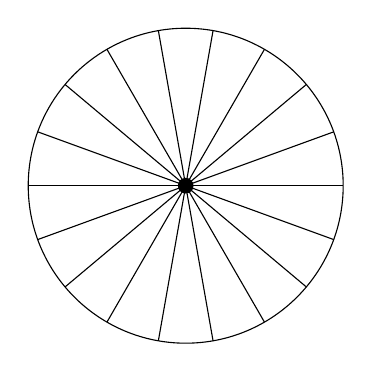
\begin{tikzpicture}
    \draw (0,0) circle (2cm);
    \foreach \x in {0,20,...,350}
    \draw[\OPTblue] (0,0) -- (\x:2cm);
    \node[\OPTblue,circle,fill,inner sep=2pt] (hub) at (0,0) {};
  \end{tikzpicture}
  \caption{由一个中心与辐条组成的二维圆盘}
  \label{fig:hub-and-spokes}
\end{figure}

我们可以利用这一思想来表达包含 $n$ 维路径构造器的高阶归纳类型,其中 $n>1$,而这些构造器仅包含一维路径构造器。
关键在于,我们可以通过一个 $(n-1)$ 维对象参数化的连续的一维路径族来获得一个 $n$ 维路径。
最简单的 $(n-1)$ 维对象是 $(n-1)$ 球面,尽管在某些情况下,一个不同的对象可能更合适。
(回顾一下,我们能够在 \cref{sec:suspension} 中使用悬挂 (suspensions) 递归地定义球面,这仅涉及一维路径构造器。
事实上,悬挂也可以看作是这种思想的一个实例,因为它涉及一个由被悬挂的类型参数化的一维路径族。)

\index{圆环}
例如,前一节中的圆环 $T^2$ 可以通过以下方式生成:
\begin{itemize}
  \item 一个点 $b:T^2$,
  \item 一条路径 $p:b=b$,
  \item 另一条路径 $q:b=b$,
  \item 一个点 $h:T^2$, 以及
  \item 对每个 $x:\Sn^1$,一条路径 $s(x) : f(x)=h$,其中 $f:\Sn^1\to T^2$ 定义为 $f(\base)\defeq b$ 和 $\ap f \lloop \defid p \ct q \ct \opp p \ct \opp q$。
\end{itemize}
这个版本的圆环的归纳原理表明,给定 $P:T^2\to\type$,对于截面 $\prd{x:T^2} P(x)$,我们需要
\begin{itemize}
  \item 一个点 $b':P(b)$,
  \item 一条路径 $p' : \dpath P p {b'} {b'}$,
  \item 一条路径 $q' : \dpath P q {b'} {b'}$,
  \item 一个点 $h':P(h)$, 以及
  \item 对每个 $x:\Sn^1$,一条路径 $\dpath {P}{s(x)}{g(x)}{h'}$,其中 $g:\prd{x:\Sn^1} P(f(x))$ 定义为 $g(\base)\defeq b'$ 和 $\apd g \lloop \defid t(p' \ct q' \ct \opp{(p')} \ct \opp{(q')})$。
  在后者中,$\ct$ 表示依赖路径的连接,$t:\eqv{(\dpath{P}{\ap f \lloop}{b'}{b'})}{(\dpath{P\circ f}{\lloop}{b'}{b'})}$ 的定义留给读者完成。
\end{itemize}
注意,不需要依赖 2-路径或 $\apdtwofunc{}$。
我们将计算规则的书写留给读者。

\begin{rmk}\label{rmk:spokes-no-hub}
有人可能会质疑引入中心点 $h$ 的必要性;为什么我们不能简单地添加连续连接圆盘边界到边界上某个点的路径,如 \cref{fig:spokes-no-hub} 所示?
然而,这在没有进一步修改的情况下是行不通的。
因为,如果给定某个 $f:\Sn^1 \to X$,我们给出一个路径构造器连接每个 $f(x)$ 到 $f(\base)$,那么我们最终得到的更像是 \cref{fig:spokes-no-hub-ii} 中的图像,一个顶点被扭曲并粘合到其底部某个点上的锥体。
问题在于,从 $f(\base)$ 到其本身的指定路径可能不是反身性 (reflexivity)。
我们可以通过添加一个 2-维路径构造器来解决这个问题,以确保这种情况,但使用一个独立的中心避免了需要任何维度超过 1 的路径构造器。
\end{rmk}

\begin{figure}
  \centering
  \begin{minipage}{2in}
    \begin{center}
      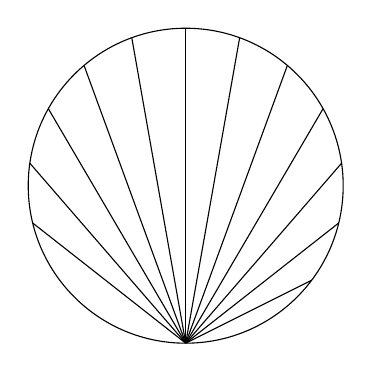
\begin{tikzpicture}
        \draw (0,0) circle (2cm);
        \clip (0,0) circle (2cm);
        \foreach \x in {0,15,...,165}
        \draw[\OPTblue] (0,-2cm) -- (\x:4cm);
      \end{tikzpicture}
    \end{center}
    \caption{无中心的辐条}
    \label{fig:spokes-no-hub}
  \end{minipage}
  \qquad
  \begin{minipage}{2in}
    \begin{center}
      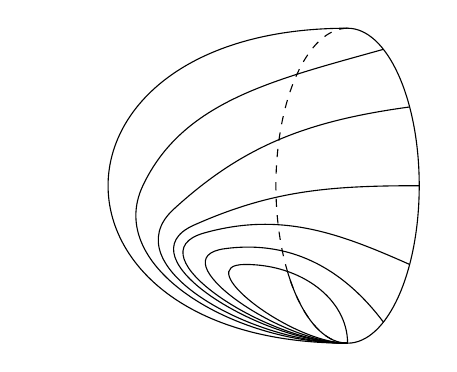
\begin{tikzpicture}[xscale=1.3]
        \draw (0,0) arc (-90:90:.7cm and 2cm) ;
        \draw[dashed] (0,4cm) arc (90:270:.7cm and 2cm) ;
        \draw[\OPTblue] (0,0) to[out=90,in=0] (-1,1) to[out=180,in=180] (0,0);
        \draw[\OPTblue] (0,4cm) to[out=180,in=180,looseness=2] (0,0);
        \path (0,0) arc (-90:-60:.7cm and 2cm) node (a) {};
        \draw[\OPTblue] (a.center) to[out=120,in=10] (-1.2,1.2) to[out=190,in=180] (0,0);
        \path (0,0) arc (-90:-30:.7cm and 2cm) node (b) {};
        \draw[\OPTblue] (b.center) to[out=150,in=20] (-1.4,1.4) to[out=200,in=180] (0,0);
        \path (0,0) arc (-90:0:.7cm and 2cm) node (c) {};
        \draw[\OPTblue] (c.center) to[out=180,in=30] (-1.5,1.5) to[out=210,in=180] (0,0);
        \path (0,0) arc (-90:30:.7cm and 2cm) node (d) {};
        \draw[\OPTblue] (d.center) to[out=190,in=50] (-1.7,1.7) to[out=230,in=180] (0,0);
        \path (0,0) arc (-90:60:.7cm and 2cm) node (e) {};
        \draw[\OPTblue] (e.center) to[out=200,in=70] (-2,2) to[out=250,in=180] (0,0);
        \clip (0,0) to[out=90,in=0] (-1,1) to[out=180,in=180] (0,0);
        \draw (0,4cm) arc (90:270:.7cm and 2cm) ;
      \end{tikzpicture}
    \end{center}
    \caption{无中心的辐条 II}
    \label{fig:spokes-no-hub-ii}
  \end{minipage}
\end{figure}

\begin{rmk}
  \index{计算规则!命题的}%
  请注意,这种将高阶路径转换为一阶路径的方法并不保留这些路径的判断计算规则,但它确实保留了命题计算规则。
\end{rmk}

\index{胞腔复形|)}%
\index{CW 复形|)}%

\index{中心与辐条|)}%


\section{推挤 (Pushouts)}
\label{sec:colimits}

\index{类型!极限}%
\index{类型!余极限}%
\index{极限!类型的极限}%
\index{余极限!类型的余极限}%
从范畴论 (category-theoretic) 的角度来看,任何基础系统的一个重要方面是构造极限 (limits) 和余极限 (colimits) 的能力。
在集合论基础中,这些是集合的极限和余极限,而在我们的情况下,它们是\emph{类型 (types)}的极限和余极限。
我们在 \cref{sec:universal-properties} 中已经看到,笛卡尔乘积类型具有类型范畴积 (categorical product of types) 的正确通用性质 (universal property),而在 \cref{ex:coprod-ump} 中,余积类型 (coproduct types) 也具有它们预期的通用性质。

如 \cref{sec:universal-properties} 中所述,可以使用等式类型 (identity types) 和 $\Sigma$ 类型来构造更一般的极限,例如 $f:A\to C$ 和 $g:B\to C$ 的纤维积 (pullback)\index{纤维积} 是 $\sm{a:A}{b:B} (f(a)=g(b))$(见 \cref{ex:pullback})。
然而,更一般的\emph{余极限}需要识别来自不同类型的元素,高阶归纳类型 (higher inductive types) 对此非常适用。
由于我们所有的构造都是同伦不变的 (homotopy-invariant),因此我们所有的余极限都是\emph{同伦余极限 (homotopy colimits)},但为了简洁起见,我们省略了无处不在的形容词。

本节我们讨论\emph{推挤 (pushouts)},作为也许最简单且最有用的余极限之一。
确实,人们期望所有有限余极限(对于一个合适的同伦定义“有限”)可以通过推挤和有限余积构造。
也可以使用高阶归纳类型直接构造更一般的余极限,但这有些技术性问题,并且不完全令人满意,因为我们尚未有一个完全通用的同伦一致图的良好概念。

\indexsee{类型!推挤}{推挤}%
\index{推挤|(defstyle}%
\index{跨 (span)}%
假设给定一个类型和函数的跨图:
\[\Ddiag=\;\vcenter{\xymatrix{C \ar^g[r] \ar_f[d] & B \\ A & }}\]
该跨图的\define{推挤 (pushout)} 是高阶归纳类型 $A\sqcup^CB$,由以下内容呈现:
\begin{itemize}
  \item 一个函数 $\inl:A\to A\sqcup^CB$,
  \item 一个函数 $\inr:B \to A\sqcup^CB$, 以及
  \item 对于每个 $c:C$,一个路径 $\glue(c):(\inl(f(c))=\inr(g(c)))$。
\end{itemize}
换句话说,$A\sqcup^CB$ 是 $A$ 和 $B$ 的不交并 (disjoint union),并且对于每个 $c:C$,有一个 $f(c)$ 和 $g(c)$ 相等的证据。
递归原理 (recursion principle) 表示,如果 $D$ 是另一个类型,我们可以通过定义以下内容来定义一个映射 $s:A\sqcup^CB\to{}D$:
\begin{itemize}
  \item 对于每个 $a:A$,$s(\inl(a))$ 的值:$D$,
  \item 对于每个 $b:B$,$s(\inr(b))$ 的值:$D$,以及
  \item 对于每个 $c:C$,$\mapfunc{s}(\glue(c))$ 的值:$s(\inl(f(c)))=s(\inr(g(c)))$。
\end{itemize}
我们将归纳原理的表述留给读者。
它还暗示了唯一性原理 (uniqueness principle),即如果 $s,s':A\sqcup^CB\to{}D$ 是两个映射,并且
\index{唯一性原理!推挤上函数的命题唯一性原理}%
\begin{align*}
  s(\inl(a))&=s'(\inl(a))\\
  s(\inr(b))&=s'(\inr(b))\\
  \mapfunc{s}(\glue(c))&=\mapfunc{s'}(\glue(c))
  \qquad\text{(基于前两个等式)}
\end{align*}
对于每个 $a,b,c$,则 $s=s'$。

为了表述推挤的通用性质 (universal property),我们引入以下定义。

\begin{defn}\label{defn:cocone}
给定一个跨图 $\Ddiag= (A \xleftarrow{f} C \xrightarrow{g} B)$ 和一个类型 $D$,在 $\Ddiag$ 下,顶点为 $D$ 的\define{余锥 (cocone)}\indexdef{余锥}%
\index{余锥的顶点}%
由函数 $i:A\to{}D$ 和 $j:B\to{}D$ 以及同伦 $h : \prd{c:C} (i(f(c))=j(g(c)))$ 组成:
\[\uppercurveobject{{ }}\lowercurveobject{{ }}\twocellhead{{ }}
\xymatrix{C \ar^g[r] \ar_f[d] \drtwocell{^h} & B \ar^j[d] \\ A \ar_i[r] & D
}\]
我们用 $\cocone{\Ddiag}{D}$ 表示所有此类余锥的类型,即
\[ \cocone{\Ddiag}{D} \defeq
\sm{i:A\to D}{j:B\to D} \prd{c:C} (i(f(c))=j(g(c))).
\]
\end{defn}

当然,存在一个在 $\Ddiag$ 下,顶点为 $A\sqcup^C B$ 的标准余锥,由 $\inl$、$\inr$ 和 $\glue$ 组成。
\[\uppercurveobject{{ }}\lowercurveobject{{ }}\twocellhead{{ }}
\xymatrix{C \ar^g[r] \ar_f[d] \drtwocell{^\glue\ \ } & B \ar^\inr[d] \\
A \ar_-\inl[r] & A\sqcup^CB }\]
以下引理表明这是通用的此类余锥。

\begin{lem}\label{thm:pushout-ump}
\index{通用性质!推挤的通用性质}%
对于任何类型 $E$,存在等价
\[ (A\sqcup^C B \to E) \;\eqvsym\; \cocone{\Ddiag}{E}. \]
\end{lem}
\begin{proof}
  我们考虑任意类型 $E:\type$。
  存在一个标准函数 $c_\sqcup$,定义如下
  \[\function{(A\sqcup^CB\to{}E)}{\cocone{\Ddiag}{E}}
  {t}{(t\circ{}\inl,t\circ{}\inr,\mapfunc{t}\circ{}\glue)}\]
  我们用非正式符号 $t\mapsto\composecocone{t}c_\sqcup$ 表示此函数。
  我们证明这是一个等价。

  首先,给定 $c=(i,j,h):\cocone{\mathscr{D}}{E}$,我们需要构造一个
  从 $A\sqcup^CB$ 到 $E$ 的映射 $\mathsf{s}(c)$。
  \[\uppercurveobject{{ }}\lowercurveobject{{ }}\twocellhead{{ }}
  \xymatrix{C \ar^g[r] \ar_f[d] \drtwocell{^h} & B \ar^{j}[d] \\
  A \ar_-{i}[r] & E }\]
  映射 $\mathsf{s}(c)$ 定义如下:
  \begin{align*}
    \mathsf{s}(c)(\inl(a))&\defeq i(a),\\
    \mathsf{s}(c)(\inr(b))&\defeq j(b),\\
    \mapfunc{\mathsf{s}(c)}(\glue(x))&\defid h(x)。
  \end{align*}
  我们定义了一个映射
  \[\function{\cocone{\Ddiag}{E}}{(A\sqcup^CB\to{}E)}{c}{\mathsf{s}(c)}\]
  我们需要证明此映射是 $t\mapsto{}\composecocone{t}c_\sqcup$ 的逆映射。
  一方面,如果 $c=(i,j,h):\cocone{\Ddiag}{E}$,我们有
  \begin{align*}
    \composecocone{\mathsf{s}(c)}c_\sqcup & =
    (\mathsf{s}(c)\circ\inl,\mathsf{s}(c)\circ\inr,
    \mapfunc{\mathsf{s}(c)}\circ\glue) \\
    & = (\lamu{a:A} \mathsf{s}(c)(\inl(a)),\;
    \lamu{b:B} \mathsf{s}(c)(\inr(b)),\;
    \lamu{x:C} \mapfunc{\mathsf{s}(c)}(\glue(x))) \\
    & = (\lamu{a:A} i(a),\;
    \lamu{b:B} j(b),\;
    \lamu{x:C} h(x)) \\
    & \jdeq (i, j, h) \\
    & = c。
  \end{align*}
%
  另一方面,如果 $t:A\sqcup^CB\to{}E$,我们想证明
  $\mathsf{s}(\composecocone{t}c_\sqcup)=t$。
  对于 $a:A$,我们有
  \[\mathsf{s}(\composecocone{t}c_\sqcup)(\inl(a))=t(\inl(a))\]
  因为 $\composecocone{t}c_\sqcup$ 的第一个分量是 $t\circ\inl$。以
  同样的方式,对于 $b:B$,我们有
  \[\mathsf{s}(\composecocone{t}c_\sqcup)(\inr(b))=t(\inr(b))\]
  对于 $x:C$,我们有
  \[\mapfunc{\mathsf{s}(\composecocone{t}c_\sqcup)}(\glue(x))
  =\mapfunc{t}(\glue(x))\]
  因此 $\mathsf{s}(\composecocone{t}c_\sqcup)=t$。

  这证明了 $c\mapsto\mathsf{s}(c)$ 是 $t\mapsto{}\composecocone{t}c_\sqcup$ 的准逆映射,正如所需。
\end{proof}

许多标准的同伦理论构造可以表示为(同伦)推挤。
\begin{itemize}
  \item 跨图 $\unit \leftarrow A \to \unit$ 的推挤是 \define{悬挂 (suspension)} $\susp A$(见 \cref{sec:suspension})。%
  \index{悬挂}
  \symlabel{join}
  \item $A \xleftarrow{\proj1} A\times B \xrightarrow{\proj2} B$ 的推挤称为 $A$ 和 $B$ 的\define{连接 (join)},记为 $A*B$。%
  \indexdef{连接!类型的连接}
  \item $\unit \leftarrow A \xrightarrow{f} B$ 的推挤称为 $f$ 的\define{锥体 (cone)}或\define{余纤维 (cofiber)}。%
  \indexdef{锥体!函数的锥体}%
  \indexsee{映射锥体}{函数的锥体}%
  \indexdef{余纤维}
  \symlabel{wedge}
  \item 如果 $A$ 和 $B$ 具有基点 (basepoints) $a_0:A$ 和 $b_0:B$,则 $A \xleftarrow{a_0} \unit \xrightarrow{b_0} B$ 的推挤是\define{楔积 (wedge)} $A\vee B$。%
  \indexdef{楔积}
  \symlabel{smash}
  \item 如果 $A$ 和 $B$ 是如前所述的有基点类型,则定义 $f:A\vee B \to A\times B$ 为 $f(\inl(a))\defeq (a,b_0)$ 和 $f(\inr(b))\defeq (a_0,b)$,其中 $\ap f \glue \defid \refl{(a_0,b_0)}$。
  那么 $f$ 的锥体称为\define{劈积 (smash product)} $A\wedge B$。%
  \indexdef{劈积}
\end{itemize}
我们将在 \cref{cha:hlevels,cha:homotopy} 中进一步讨论推挤。

\begin{rmk}
  正如在 \cref{subsec:prop-trunc} 中所述,对于有基点的空间,劈积和楔积的符号 $\wedge$ 和 $\vee$ 也用于逻辑中的“与 (and)”和“或 (or)”。
  由于同伦类型论中的类型既可以表现得像空间,也可以表现得像命题,因此存在冲突的潜在可能性——但由于它们很少同时这样做,通常上下文可以消除歧义。
  此外,劈积和楔积仅适用于\emph{有基点}的空间,而唯一的有基点的纯命题是 $\top\jdeq\unit$——并且我们有 $\unit\wedge \unit = \unit$ 和 $\unit\vee\unit=\unit$ 对于 $\wedge$ 和 $\vee$ 的任何含义都成立。
\end{rmk}

\index{推挤|)}%

\begin{rmk}
  请注意,余极限通常不保留截断性 (truncatedness)。
  例如,$\Sn^0$ 和 \unit 都是集合 (sets),但 $\unit \leftarrow \Sn^0 \to \unit$ 的推挤是 $\Sn^1$,它不是集合。
  因此,如果我们对 $n$-类型范畴 (category of $n$-types) 中的余极限感兴趣(特别是在集合的范畴中),我们需要以某种方式“截断”余极限。
  我们将在 \cref{sec:hittruncations,cha:hlevels,cha:set-math} 中回到这一点。
\end{rmk}

\section{截断 (Truncations)}
\label{sec:hittruncations}

\index{截断!命题截断|(propositional truncation|(}%
在\cref{subsec:prop-trunc}中,我们介绍了命题截断 (propositional truncation) 作为一种新的类型构造操作;现在我们发现它可以作为高阶归纳类型 (higher inductive types) 的一种特殊情况来获得。这将理解截断的问题简化为理解高阶归纳类型的问题,而高阶归纳类型至少是可以系统处理的。这个现象也很有趣,因为它为我们提供了第一个真正\emph{递归 (recursive)} 的高阶归纳类型的例子,即它的构造器从正在定义的类型中获取输入(就像后继 $\suc:\nat\to\nat$ 一样)。

设 $A$ 是一个类型;我们定义其命题截断 $\brck A$ 为由以下构造器生成的高阶归纳类型:
\begin{itemize}
  \item 一个函数 $\bprojf : A \to \brck A$,以及
  \item 对于每个 $x,y:\brck A$,一个路径 $x=y$。
\end{itemize}
请注意,第二个构造器实际上是断言 $\brck A$ 是一个纯命题 (mere proposition)。因此,$\brck A$ 的定义可以解释为 $\brck A$ 是由 $A\to\brck A$ 的函数和它是一个纯命题的事实自由生成的。

该高阶归纳定义的递归原理 (recursion principle) 很容易写出来:它表示给定任意类型 $B$,以及
\begin{itemize}
  \item 一个函数 $g:A\to B$,以及
  \item 对于任意 $x,y:B$,一个路径 $x=_B y$,
\end{itemize}
存在一个函数 $f:\brck A \to B$ 使得
\begin{itemize}
  \item 对于所有 $a:A$,$f(\bproj a) \jdeq g(a)$,以及
  \item 对于任意 $x,y:\brck A$,函数 $\apfunc f$ 将 $\brck A$ 中指定的路径 $x=y$ 映射到 $B$ 中指定的路径 $f(x) = f(y)$(命题性地)。
\end{itemize}
\index{递归原理!截断的递归原理}%
这些正是我们在\cref{subsec:prop-trunc}中为命题截断的递归原理所陈述的假设——一个 $A\to B$ 的函数,且 $B$ 是一个纯命题——结论的第一部分正是我们在那里陈述的内容。结论的第二部分($\apfunc f$ 的作用)之前没有提到,但在这种情况下是空洞的,因为 $B$ 是一个纯命题,所以\emph{任何}两条路径在其中都自动相等。

\index{归纳原理!截断的归纳原理}%
$\brck A$ 还有一个归纳原理 (induction principle),它表示给定任意 $B:\brck A \to \type$ 以及
\begin{itemize}
  \item 一个函数 $g:\prd{a:A} B(\bproj a)$,以及
  \item 对于任意 $x,y:\brck A$ 和 $u:B(x)$ 以及 $v:B(y)$,一个依赖路径 $q:\dpath{B}{p(x,y)}{u}{v}$,其中 $p(x,y)$ 是从 $\brck A$ 的第二个构造器中获得的路径,
\end{itemize}
存在 $f:\prd{x:\brck A} B(x)$ 使得 $f(\bproj a)\jdeq g(a)$ 对于 $a:A$ 成立,并且还有另一个计算规则。然而,由于在任何两个纯命题之间至多可以存在一个函数(最多到同伦),这个归纳原理并没有太大用处(参见\cref{ex:prop-trunc-ind})。

\index{截断!命题截断|)}%
\index{截断!集合|(set truncation|)}%

\index{集合|(set|(}%
我们可以扩展这个想法来构造类似的截断,落在 $n$-类型中,对于任意 $n$。例如,我们可以定义\emph{0-截断 (0-truncation)} $\trunc0A$ 为由以下内容生成的:
\begin{itemize}
  \item 一个函数 $\tprojf0 : A \to \trunc0 A$,以及
  \item 对于每个 $x,y:\trunc0A$ 和每个 $p,q:x=y$,一个路径 $p=q$。
\end{itemize}
然后 $\trunc0A$ 将由一个 $A\to \trunc0A$ 的函数以及 $\trunc0A$ 是一个集合 (set) 的断言自由生成。它的一个自然的归纳原理表示,给定 $B:\trunc0 A \to \type$ 以及
\begin{itemize}
  \item 一个函数 $g:\prd{a:A} B(\tproj0a)$,以及
  \item 对于任意 $x,y:\trunc0A$,以及 $z:B(x)$ 和 $w:B(y)$,以及每个 $p,q:x=y$ 和 $r:\dpath{B}{p}{z}{w}$ 以及 $s:\dpath{B}{q}{z}{w}$,一个 $v:\dpath{\dpath{B}{-}{z}{w}}{u(x,y,p,q)}{r}{s}$ 的2路径,其中 $u(x,y,p,q):p=q$ 是从 $\trunc0A$ 的第二个构造器中获得的,
\end{itemize}
存在 $f:\prd{x:\trunc0A} B(x)$ 使得 $f(\tproj0a)\jdeq g(a)$ 对于所有 $a:A$ 成立,并且 $\apdtwo{f}{u(x,y,p,q)}$ 是上面指定的2路径。(如同命题情况,后者的条件被证明是不太重要的。)然而,从这可以证明一个更有用的归纳原理。

\begin{lem}\label{thm:trunc0-ind}
假设给定 $B:\trunc0 A \to \type$ 以及 $g:\prd{a:A} B(\tproj0a)$,并假设每个 $B(x)$ 是一个集合。然后存在 $f:\prd{x:\trunc0A} B(x)$ 使得 $f(\tproj0a)\jdeq g(a)$ 对于所有 $a:A$ 成立。
\end{lem}
\begin{proof}
  只需为上述的任意 $x,y,z,w,p,q,r,s$ 构造一个2路径 $v:\dpath{B}{u(x,y,p,q)}{r}{s}$ 即可。然而,根据依赖2路径的定义,这只是 $B(y)$ 中的一个普通2路径。由于 $B(y)$ 是一个集合,因此在任何两个平行路径之间都存在一个2路径。
\end{proof}

这暗示了预期的通用性质。

\begin{lem}\label{thm:trunc0-lump}
\index{通用性质!截断的通用性质}%
对于任意集合 $B$ 和任意类型 $A$,与 $\tprojf0:A\to \trunc0A$ 组合的合成决定了一个等价
\[ \eqvspaced{(\trunc0A\to B)}{(A\to B)}。 \]
\end{lem}
\begin{proof}
  当 $B$ 是常数族时,\cref{thm:trunc0-ind} 的特例提供了一个从右到左的映射,它是从左到右的“与 $\tprojf0$ 组合”函数的右逆。
  要证明它也是左逆,设 $h:\trunc0A\to B$,并通过将\cref{thm:trunc0-ind} 应用于复合 $a\mapsto h(\tproj0a)$ 来定义 $h':\trunc0A\to B$。因此,对于任意 $a:A$,$h'(\tproj0a)=h(\tproj0a)$。

  然而,由于 $B$ 是一个集合,对于任意 $x:\trunc0A$,类型 $h(x)=h'(x)$ 是一个纯命题,因此也是一个集合。因此,依据\cref{thm:trunc0-ind},观察到 $h'(\tproj0a)=h(\tproj0a)$ 对于任意 $a:A$ 表明对于任意 $x:\trunc0A$,$h(x)=h'(x)$,因此 $h=h'$。
\end{proof}

\index{集合的极限}%
\index{集合的余极限}%
例如,这使我们能够构造集合的余极限。我们已经看到,如果 $A \xleftarrow{f} C \xrightarrow{g} B$ 是一组集合,则推挤 $A\sqcup^C B$ 可能不再是一个集合。(例如,如果 $A$ 和 $B$ 是 \unit 而 $C$ 是 \bool,则推挤是 $\Sn^1$。)然而,我们可以通过截断构造一个集合的推挤,并具有与其他集合相关的预期通用性质。

\begin{lem}\label{thm:set-pushout}
\index{通用性质!推挤的通用性质}%
设 $A \xleftarrow{f} C \xrightarrow{g} B$ 是一组集合。则对于任意集合 $E$,存在一个典型的等价
\[ \Parens{\trunc0{A\sqcup^C B} \to E} \;\eqvsym\; \cocone{\Ddiag}{E}。 \]
\end{lem}
\begin{proof}
  结合\cref{thm:pushout-ump,thm:trunc0-lump} 中的等价性。
\end{proof}

我们将 $\trunc0{A\sqcup^C B}$ 称为\define{集合推挤 (set-pushout)}%
\indexdef{集合推挤}%
\index{推挤!集合的推挤}的 $f$ 和 $g$,以将其与(同伦)推挤 $A\sqcup^C B$ 区分开来。或者,我们可以直接修改\cref{sec:colimits} 中的推挤定义,以包括0截断构造器,从而避免事后截断。类似的备注也适用于任何类型的集合余极限;我们将在\cref{cha:set-math} 中进一步探讨这个问题。

然而,虽然上述的0截断定义是可行的——它给出了我们想要的结果,并且是一致的——它有几个问题。首先,它不太适合高阶归纳类型的一般理论。通常,直接处理像我们为 $\trunc0A$ 给出的第二个构造器这样的构造器是很棘手的,因为它们的\emph{输入}不仅涉及正在定义的类型中的元素,还涉及其中的路径。

然而,这个问题可以相当容易地解决。回想一下,在\cref{sec:bool-nat} 中我们提到,我们可以通过让构造器获取一个类型 $W$ 的归纳类型 $W$ 的“无限多的参数”,从而允许一个构造器接受无限多个 $W$ 类型的参数,例如通过让它获取类型 $\nat\to W$ 的单个参数。这背后有一个普遍的原则:为了模拟具有奇特输入的构造器,使用辅助归纳类型(如 \nat)对它们进行参数化,将输入简化为具有归纳域的简单函数。

对于0截断,我们可以考虑辅助的\emph{高阶}归纳类型 $S$,它由两个点 $a,b:S$ 和两条路径 $p,q:a=b$ 生成。然后,$\trunc 0A$ 中看似奇怪的构造器可以被替换为无可非议的
\begin{itemize}
  \item 对于每个 $f:S\to \trunc 0A$,一条路径 $\apfunc{f}(p) = \apfunc{f}(q)$。
\end{itemize}
因为给定 $S$ 的映射等同于给出两个点和它们之间的两条平行路径,这将产生相同的归纳原理。

\index{集合|)}%

\index{截断!集合截断|)}%
\index{截断!n-截断@$n$-截断}%
然而,我们当前的0截断定义的一个更严重的问题是,它不能很好地推广。如果我们想描述一个统一定义的“$n$-截断”到 $n$-类型中的概念,对于任意 $n:\nat$,那么这种方法是不可行的,因为第二个构造器需要的参数数量随着 $n$ 的增加而增加。因此,在\cref{sec:truncations} 中,我们将使用一个不同的想法来构造这些,基于一个观察,即上述引入的类型 $S$ 等价于圆 $\Sn^1$。这包括了0截断作为一个特殊情况,并满足\cref{thm:trunc0-ind,thm:trunc0-lump} 的广义版本。


\section{商 (Quotients)}
\label{sec:set-quotients}

集合的一种特别重要的余极限是通过关系的\emph{商 (quotient)}。也就是说,设 $A$ 是一个集合,$R:A\times A \to \prop$ 是一族纯命题(\define{纯关系 (mere relation)})。\indexdef{关系!纯关系}%
\indexdef{纯关系}%
它的商应该是以下两个投影的集合并等化子 (set-coequalizer)
\[ \tsm{a,b:A} R(a,b) \rightrightarrows A。 \]
我们也可以直接描述它,作为由以下内容生成的高阶归纳类型 $A/R$:
\index{集合商|(defstyle}%
\indexsee{集合的商}{集合商}%
\indexsee{类型的商}{集合商}%
\begin{itemize}
  \item 一个函数 $q:A\to A/R$;
  \item 对于每个 $a,b:A$,如果 $R(a,b)$,则有一个等式 $q(a)=q(b)$;以及
  \item 0截断构造器:对于所有 $x,y:A/R$ 和 $r,s:x=y$,我们有 $r=s$。
\end{itemize}
我们有时会将这个高阶归纳类型 $A/R$ 称为 $A$ 关于 $R$ 的\define{集合商},以强调它按定义生成了一个集合。(在同伦理论中有更一般的“商”概念,但它们大多超出了本书的范围。然而,在\cref{sec:rezk} 中,我们将考虑一个类型关于1-群胚 (1-groupoid) 的“商”,这是集合商之上的下一个层次。)

\begin{rmk}\label{rmk:quotient-of-non-set}
事实上,定义集合商时,并不需要 $A$ 是一个集合。尽管如此,这通常是最感兴趣的情况。
\end{rmk}

\begin{lem}\label{thm:quotient-surjective}
函数 $q:A\to A/R$ 是满射。
\end{lem}
\begin{proof}
  我们必须证明,对于任意 $x:A/R$,存在一个 $a:A$ 使得 $q(a)=x$。我们使用 $A/R$ 的归纳原理。第一个情况是显然的:如果 $x$ 是 $q(a)$,那么当然存在一个 $a$,使得 $q(a)=q(a)$。由于目标是一个纯命题,它自动尊重所有路径构造器,因此我们完成了证明。
\end{proof}

现在我们可以证明集合商具有预期的集合并等化子的通用性质。

\begin{lem}\label{thm:quotient-ump}
对于任意集合 $B$,预合成 $q$ 得到一个等价
\[ \eqvspaced{(A/R \to B)}{\Parens{\sm{f:A\to B} \prd{a,b:A} R(a,b) \to (f(a)=f(b))}}。 \]
\end{lem}
\begin{proof}
  从右到左的 $\blank\circ q$ 的准逆是 $A/R$ 的递归原理。也就是说,给定 $f:A\to B$,使得
  \narrowequation{\prd{a,b:A} R(a,b) \to (f(a)=f(b)),} 我们通过定义 $\bar f:A/R\to B$ 为 $\bar f(q(a))\defeq f(a)$。
  这个定义等式正好说明了 $(f\mapsto \bar f)$ 是 $(\blank\circ q)$ 的右逆。

  为了证明它也是左逆,我们必须证明,对于任意 $g:A/R\to B$ 和 $x:A/R$,我们有 $g(x) = \overline{g\circ q}(x)$。
  然而,根据\cref{thm:quotient-surjective},仅存在一个 $a$ 使得 $q(a)=x$。由于我们想要的等式是一个纯命题,我们可以假设确实存在这样的 $a$,在这种情况下,$g(x) = g(q(a)) = \overline{g\circ q}(q(a)) = \overline{g\circ q}(x)$。
\end{proof}

当然,经典情况下通常考虑 $R$ 是一个\define{等价关系 (equivalence relation)},即我们有
\indexdef{关系!等价}%
\indexsee{等价!关系}{关系, 等价}%
%
\begin{itemize}
  \item \define{自反性 (reflexivity)}:$\prd{a:A} R(a,a)$,
  \indexdef{自反性!关系的自反性}%
  \indexdef{关系!自反性}%
  \item \define{对称性 (symmetry)}:$\prd{a,b:A} R(a,b) \to R(b,a)$,以及
  \indexdef{对称性!关系的对称性}%
  \indexdef{关系!对称性}%
  \item \define{传递性 (transitivity)}:$\prd{a,b,c:C} R(a,b) \times R(b,c) \to R(a,c)$。
  \indexdef{传递性!关系的传递性}%
  \indexdef{关系!传递性}%
\end{itemize}
%
在这种情况下,集合商 $A/R$ 具有额外的良好性质,正如我们将在\cref{sec:piw-pretopos} 中看到的:例如,我们有 $R(a,b) \eqvsym (\id[A/R]{q(a)}{q(b)})$。
\symlabel{等价关系}
我们通常将等价关系 $R(a,b)$ 以中缀形式写为 $a\eqr b$。

等价关系的商也可以通过其他方式构造。集合论的方法是将等价类视为幂集\index{幂集} $A$ 的子集。我们也可以在类型论中模仿这种“泛型 (impredicative)”构造。
\index{泛型!商}

\begin{defn}
  如果对于任意 $b:A$ 我们有 $\eqv{R(a,b)}{P(b)}$,则谓词 $P:A\to\prop$ 是关系 $R : A \times A \to \prop$ 的\define{等价类 (equivalence class)}。
\end{defn}

由于 $R$ 和 $P$ 是纯命题,等价 $\eqv{R(a,b)}{P(b)}$ 等同于蕴涵 $R(a,b) \to P(b)$ 和 $P(b) \to R(a,b)$。当然,对于任意 $a:A$,我们有规范的等价类 $P_a(b) \defeq R(a,b)$。

\begin{defn}\label{def:VVquotient}
我们定义
\begin{equation*}
  A\sslash R \defeq \setof{ P:A\to\prop | P \text{ 是 } R \text{ 的一个等价类}}。
\end{equation*}
函数 $q':A\to A\sslash R$ 定义为 $q'(a) \defeq P_a$。
\end{defn}

\begin{thm}
  对于任意集合 $A$ 上的等价关系 $R$,类型 $A\sslash R$ 与集合商 $A/R$ 等价。
\end{thm}
\begin{proof}
  首先注意,如果 $R(a,b)$,则由于 $R$ 是等价关系,对于任意 $c:A$,我们有 $R(a,c) \Leftrightarrow R(b,c)$。因此,通过一值性 (univalence),$R(a,c) = R(b,c)$,因此通过函数扩展性 (function extensionality),$P_a=P_b$,即 $q'(a)=q'(b)$。因此,根据\cref{thm:quotient-ump},我们有一个从 $A/R$ 到 $A\sslash R$ 的诱导映射 $f$,使得 $f\circ q = q'$。

  我们证明 $f$ 是单射且满射,因此是一个等价。满射性直接来自 $q'$ 的满射性,后者本质上是由 $A\sslash R$ 的定义决定的。对于单射性,如果 $f(x)=f(y)$,则为了证明纯命题 $x=y$,通过 $q$ 的满射性,我们可以假设 $x=q(a)$ 和 $y=q(b)$ 对于某些 $a,b:A$。然后,对于任意 $c:A$,$R(a,c) = f(q(a))(c) = f(q(b))(c) = R(b,c)$,特别地,$R(a,b) = R(b,b)$。但是 $R(b,b)$ 是有元素的,因为 $R$ 是等价关系,因此 $R(a,b)$ 也是有元素的。因此 $q(a)=q(b)$,因此 $x=y$。
\end{proof}

在\cref{subsec:quotients} 中,我们将给出该定理的另一种证明。注意,与 $A/R$ 不同,构造 $A\sslash R$ 提升了宇宙层次:如果 $A:\UU_i$ 且 $R:A\to A\to \prop_{\UU_i}$,则在 $A\sslash R$ 的定义中,我们还必须使用 $\prop_{\UU_i}$ 来包含所有等价类,因此 $A\sslash R : \UU_{i+1}$。当然,如果我们假设来自\cref{subsec:prop-subsets} 的命题重缩放公理 (propositional resizing axiom),我们可以避免这个问题。

\begin{rmk}\label{defn-Z}
之前的两个构造提供了普遍的商,但在特殊情况下,可能存在更简单的构造。例如,我们可以定义整数 \Z 作为集合商
\indexdef{整数}%
\indexdef{数字!整数}%
%
\[ \Z \defeq (\N \times \N)/{\eqr} \]
%
其中 $\eqr$ 是通过以下方式定义的等价关系:
%
\[ (a,b) \eqr (c,d) \defeq (a + d = b + c)。 \]
%
换句话说,一个对 $(a,b)$ 代表整数 $a - b$。然而,在这种情况下存在\emph{规范的代表 (canonical representatives)}:即形如 $(n,0)$ 或 $(0,n)$ 的代表。
\end{rmk}

以下引理表明,当出现这种情况时,我们不需要任一一般商的构造。(一个函数 $r:A\to A$ 称为\define{幂等的 (idempotent)}%
\indexdef{函数!幂等的}%
\indexdef{幂等的!函数}%
当且仅当 $r\circ r = r$。)

\begin{lem}\label{lem:quotient-when-canonical-representatives}
假设 $\eqr$ 是集合 $A$ 上的关系,并且存在一个幂等 $r:A \to A$,使得对于所有 $x,y: A$,$\eqv{(r(x) = r(y))}{(x \eqr y)}$。(这意味着 $\eqr$ 是一个等价关系。)那么类型
%
\begin{equation*}
(A/{\eqr}) \defeq \Parens{\sm{x : A} r(x) = x}
\end{equation*}
%
满足 $A$ 关于 $\eqr$ 的集合商的通用性质,因此与之等价。换句话说,有一个映射 $q : A \to (A/{\eqr})$,使得对于每个集合 $B$,与 $q$ 的预合成诱导一个等价
%
\begin{equation}
  \label{eq:quotient-when-canonical}
  \Parens{(A/{\eqr}) \to B} \eqvsym \Parens{\sm{g : A \to B} \prd{x, y : A} (x \eqr y) \to (g(x) = g(y))}。
\end{equation}
\end{lem}

\begin{proof}
  设 $i:\prd{x : A} r(r(x)) = r(x)$ 见证了 $r$ 的幂等性。映射 $q:A\to (A/{\eqr})$ 定义为 $q(x) \defeq (r(x), i(x))$。注意,由于 $A$ 是一个集合,我们有 $q(x)=q(y)$ 当且仅当 $r(x)=r(y)$,因此(根据假设)当且仅当 $x \eqr y$。我们通过以下方式定义~\eqref{eq:quotient-when-canonical} 中从左到右的映射 $e$:
  \[ e(f) \defeq (f \circ q, \nameless) \]
  %
  其中下划线 $\nameless$ 表示以下证明:如果 $x, y : A$ 并且 $x \eqr y$,则 $q(x)=q(y)$ 如上所述,因此 $f(q(x)) = f(q(y))$。
  为了证明 $e$ 是一个等价,考虑由以下方式定义的相反方向的映射 $e'$:
  %
  \[ e'(g, s) (x,p) \defeq g(x)。 \]
  %
  给定任意 $f : (A/{\eqr}) \to B$,
  %
  \[ e'(e(f))(x, p) \jdeq f(q(x)) \jdeq f(r(x), i(x)) = f(x, p) \]
  %
  因为最后的等式成立是因为 $p : r(x) = x$,因此 $(x,p) = (r(x), i(x))$ 因为 $A$ 是一个集合。类似地我们计算
  %
  \[ e(e'(g, s)) \jdeq e(g \circ \proj{1}) \jdeq (g \circ \proj{1} \circ q, {\nameless})。 \]
  %
  因为 $B$ 是一个集合,我们不必担心 $\nameless$ 部分,而对于第一个分量,我们有
  %
  \[ g(\proj{1}(q(x))) \jdeq g(r(x)) = g(x), \]
  %
  其中最后一个等式成立是因为 $r(x) \eqr x$,并且 $g$ 尊重 $s$ 所假设的 $\eqr$。
\end{proof}

\begin{cor}\label{thm:retraction-quotient}
假设 $p:A\to B$ 是一个集合之间的收缩映射 (retraction)。那么 $B$ 是 $A$ 关于等价关系 $\eqr$ 的商,$\eqr$ 定义为
\[ (a_1 \eqr a_2) \defeq (p(a_1) = p(a_2))。 \]
\end{cor}
\begin{proof}
  假设 $s:B\to A$ 是 $p$ 的一个截面 (section)。然后 $s\circ p : A\to A$ 是一个满足\cref{lem:quotient-when-canonical-representatives} 的 $\eqr$ 的幂等,并且 $s$ 诱导了 $B$ 到其固定点集的同构。
\end{proof}

\begin{rmk}\label{Z-quotient-by-canonical-representatives}
\cref{lem:quotient-when-canonical-representatives} 适用于 $\Z$,使用定义的幂等 $r : \N \times \N \to \N \times \N$
定义为
%
\begin{equation*}
  r(a, b) =
  \begin{cases}
  (a - b, 0) & \text{如果 } a \geq b,\\
  (0, b - a) & \text{否则。}
  \end{cases}
\end{equation*}
%
(即使在构造上这个定义也是有效的,因为 $\N$ 上的关系 $\geq$ 是可判定的。)因此,一个非负整数被规范地表示为 $(k, 0)$,一个非正整数表示为 $(0, m)$,其中 $k,m:\N$。这个分案例表示了以下整数的“归纳原理 (induction principle)”。
\index{自然数}%
(如往常一样,我们将自然数 $n$ 识别为对应的非负整数,即 $(n,0):\N\times\N$ 在 $\Z$ 中的像。)
\end{rmk}

\begin{lem}\label{thm:sign-induction}
\index{整数!整数的归纳原理}%
\index{归纳原理!整数的归纳原理}%
假设 $P:\Z\to\type$ 是一个类型族,并且我们有
\begin{itemize}
  \item $d_0: P(0)$,
  \item $d_+: \prd{n:\N} P(n) \to P(\suc(n))$,以及
  \item $d_- : \prd{n:\N} P(-n) \to P(-\suc(n))$。
\end{itemize}
那么我们有 $f:\prd{z:\Z} P(z)$ 使得
\begin{itemize}
  \item $f(0) = d_0$,
  \item 对于所有 $n:\N$,$f(\suc(n)) = d_+(n,f(n))$,以及
  \item 对于所有 $n:\N$,$f(-\suc(n)) = d_-(n,f(-n))$。
\end{itemize}
\end{lem}
\begin{proof}
  为了证明此引理,我们让 $\Z$ 表示 $\sm{x:\N\times\N}(r(x)=x)$,其中 $r$ 是上述的幂等。(然后我们可以将结果传递到与 $\Z$ 等价的任何定义。) 让 $q:\N\times\N\to\Z$ 是商映射,定义为 $q(x) = (r(x),i(x))$,如\cref{lem:quotient-when-canonical-representatives} 中所述。现在定义 $Q\defeq P\circ q:\N\times \N \to \type$。通过跨越适当的等式传递给定的数据,我们得到
  \begin{align*}
    d'_0 &: Q(0,0)\\
    d'_+ &: \prd{n:\N} Q(n,0) \to Q(\suc(n),0)\\
    d'_- &: \prd{n:\N} Q(0,n) \to Q(0,\suc(n))。
  \end{align*}
  还注意,由于 $q(n,m) = q(\suc(n),\suc(m))$,我们有一个诱导等价
  \[e_{n,m}:\eqv{Q(n,m)}{Q(\suc(n),\suc(m))}。]
  然后我们通过双重归纳在 $x$ 上构造 $g:\prd{x:\N\times \N} Q(x)$:
  \begin{align*}
    g(0,0) &\defeq d'_0,\\
    g(\suc(n),0) &\defeq d'_+(n,g(n,0)),\\
    g(0,\suc(m)) &\defeq d'_-(m,g(0,m)),\\
    g(\suc(n),\suc(m)) &\defeq e_{n,m}(g(n,m))。
  \end{align*}
  现在我们有 $\proj1 : \Z \to \N\times\N$,其属性为 $q\circ \proj1 = \idfunc$。特别地,因此我们有 $Q\circ \proj1 = P$,因此有一组等价 $s:\prd{z:\Z} \eqv{Q(\proj1(z))}{P(z)}$。因此,我们可以定义 $f(z) = s(z,g(\proj1(z)))$ 以获得 $f:\prd{z:\Z} P(z)$,并验证所需的等式。
\end{proof}

我们有时会用模式匹配语法表示从\cref{thm:sign-induction} 获得的函数 $f:\prd{z:\Z} P(z)$,涉及三种情况 $d_0$,$d_+$ 和 $d_-$:
\begin{align*}
  f(0) &\defid d_0\\
  f(\suc(n)) &\defid d_+(n,f(n))\\
  f(-\suc(n)) &\defid d_-(n,f(-n))
\end{align*}
我们使用 $\defid$ 而不是 $\defeq$,就像我们对高阶归纳类型的路径构造器所做的那样,表示由\cref{thm:sign-induction} 隐含的“计算”规则只是命题性等式。例如,通过这种方式我们可以定义任意整数 $n$ 的 $n$ 倍连接环 (n-fold concatenation of a loop)。

\begin{cor}\label{thm:looptothe}
\indexdef{路径!连接!n倍连接@$n$-倍连接}%
设 $A$ 是一个具有 $a:A$ 和 $p:a=a$ 的类型。存在一个函数 $\prd{n:\Z} (a=a)$,记作 $n\mapsto p^n$,定义为
\begin{align*}
  p^0 &\defid \refl{a}\\
  p^{n+1} &\defid p^n \ct p
  & &\text{对于 $n\ge 0$}\\
  p^{n-1} &\defid p^n \ct \opp p
  & &\text{对于 $n\le 0$。}
\end{align*}
\end{cor}

我们将在\cref{sec:free-algebras,sec:field-rati-numb} 中进一步讨论整数。

\index{集合商|)}%

\section{代数 (Algebra)}
\label{sec:free-algebras}

除了构造球面和胞腔复形 (cell complexes) 这样的高维对象外,即使仅在集合上工作,高阶归纳类型 (higher inductive types) 也非常有用。我们在 \cref{thm:set-pushout} 中已经看到了一个例子:它们允许我们构造任何集合图的余极限 (colimit),而这是在 \cref{cha:typetheory} 的基础类型论中无法实现的。当我们研究具有代数结构的集合时,高阶归纳类型也非常有用。

在本节中,我们将以\emph{群 (groups)} 作为一个持续的例子,这对于大多数数学家来说是熟悉的,并展示了基本现象(在后续章节中也将需要它们)。然而,我们所说的大部分内容同样适用于任何形式的代数结构。

\index{幺半群|(}%

\begin{defn}
  \define{幺半群 (monoid)}
  \indexdef{monoid}%
  是一个集合 $G$ 以及
  \begin{itemize}
    \item 一个\emph{乘法 (multiplication)}
    \indexdef{multiplication!in a monoid}%
    \indexdef{multiplication!in a group}%
    函数 $G\times G\to G$,写作中缀形式 $(x,y) \mapsto x\cdot y$;以及
    \item 一个\emph{单位元 (unit)}
    \indexdef{unit!of a monoid}%
    \indexdef{unit!of a group}%
    元素 $e:G$;使得
    \item 对于任意 $x:G$,我们有 $x\cdot e = x$ 且 $e\cdot x = x$;以及
    \item 对于任意 $x,y,z:G$,我们有 $x\cdot (y\cdot z) = (x\cdot y)\cdot z$。
    \index{associativity!in a monoid}%
    \index{associativity!in a group}%
  \end{itemize}
  \define{群 (group)}
  \indexdef{group}%
  是一个幺半群 $G$,并且
  \begin{itemize}
    \item 一个\emph{逆元 (inversion)} 函数 $i:G\to G$,写作 $x\mapsto \opp x$;使得
    \index{inverse!in a group}%
    \item 对于任意 $x:G$ 我们有 $x\cdot \opp x = e$ 且 $\opp x \cdot x = e$。
  \end{itemize}
\end{defn}

\begin{rmk}\label{rmk:infty-group}
注意,我们要求群是一个集合。我们可以考虑一种更一般的“$\infty$-群 ($\infty$-group)”%
\index{.infinity-group@$\infty$-group}
它不一定是一个集合,但这会让我们偏离当前的讨论主题。在我们的定义中,我们可以期望所得到的“群论”表现得与集合论数学中的方式类似(除非我们假设 \LEM{},否则它将是“构造性的”群论 (constructive group theory))。\index{mathematics!constructive}
\end{rmk}

\begin{eg}
  自然数 \N 在加法下是一个幺半群,单位元是 $0$,在乘法下也是一个幺半群,单位元是 $1$。如果我们以显而易见的方式定义整数 \Z 上的算术运算,那么通常它们在加法下是一个群,在乘法下是一个幺半群(当然,它们也是一个环)。例如,如果 $u, v \in \Z$ 分别表示为 $(a,b)$ 和 $(c,d)$,那么 $u + v$ 表示为 $(a + c, b + d)$,$-u$ 表示为 $(b, a)$,而 $u v$ 表示为 $(a c + b d, a d + b c)$。
\end{eg}

\begin{eg}\label{thm:homotopy-groups}
我们在 \cref{sec:equality} 中实质上观察到,如果 $(A,a)$ 是一个尖点类型 (pointed type),那么它的循环空间 (loop space)\index{loop space} $\Omega(A,a)\defeq (\id[A]aa)$ 具有群的所有结构,除了它通常不是一个集合。它应该是 \cref{rmk:infty-group} 中提到的“$\infty$-群”,但我们也可以通过截断 (truncation) 使它成为一个群。具体地,我们定义 $A$ 在点 $a:A$ 处的 \define{基本群 (fundamental group)}
\indexsee{group!fundamental}{fundamental group}%
\indexdef{fundamental!group}%
为
\[\pi_1(A,a)\defeq \trunc0{\Omega(A,a)}。\]
这继承了一个群结构;例如,通过对路径的连接进行双重截断,定义了乘法 $\pi_1(A,a) \times \pi_1(A,a) \to \pi_1(A,a)$。

更一般地,$(A,a)$ 的 \define{$n$ 阶同伦群 (homotopy group)}
\index{homotopy!group}%
\indexsee{group!homotopy}{homotopy group}%
定义为 $\pi_n(A,a)\defeq \trunc0{\Omega^n(A,a)}$。
\index{loop space!iterated}%
因此对于 $n\ge 1$,有 $\pi_n(A,a) = \pi_1(\Omega^{n-1}(A,a))$,所以它也是一个群。(当 $n=0$ 时,我们有 $\pi_0(A) \jdeq \trunc0 A$,它不是一个群。)此外,Eckmann-Hilton 论证 \index{Eckmann--Hilton argument} (\cref{thm:EckmannHilton}) 表明,如果 $n\ge 2$,则 $\pi_n(A,a)$ 是一个\emph{阿贝尔群 (abelian group)},即对于所有 $x,y$ 有 $x\cdot y = y\cdot x$。\cref{cha:homotopy} 将主要研究这些群。
\end{eg}

\index{algebra!free}%
\index{free!algebraic structure}%
群论中的一个重要概念是由一个集合生成的\emph{自由群 (free group)},或更一般地,由生成元 (generators)\index{generator!of a group} 和关系 (relations) 表示的群。众所周知,在类型论中,\emph{一些} 自由代数对象可以使用\emph{普通的}归纳类型 (inductive types) 定义。
\symlabel{lst-freemonoid}%
\indexdef{type!of lists}%
\indexsee{list type}{type, of lists}%
\index{monoid!free|(}%
例如,集合 $A$ 上的自由幺半群可以与 $A$ 元素的\emph{有限列表 (finite lists)} 类型 $\lst A$ 进行标识,后者通过归纳生成:
\begin{itemize}
  \item 构造函数 $\nil:\lst A$,以及
  \item 对于每个 $\ell:\lst A$ 和 $a:A$,生成一个元素 $\cons(a,\ell):\lst A$。
\end{itemize}
我们有一个显然的包含 $\eta : A\to \lst A$,定义为 $a\mapsto \cons(a,\nil)$。$\lst A$ 上的幺半群运算是连接 (concatenation),递归定义为
\begin{align*}
  \nil \cdot \ell &\defeq \ell\\
  \cons (a,\ell_1) \cdot \ell_2 &\defeq \cons(a, \ell_1\cdot\ell_2)。
\end{align*}
使用 $\lst A$ 的归纳原理可以很容易地证明 $\lst A$ 是一个集合,并且列表的连接是结合的 (associative)
\index{associativity!of list concatenation}%
并且 $\nil$ 作为单位元。因此,$\lst A$ 是一个幺半群。

\begin{lem}\label{thm:free-monoid}
\indexsee{free!monoid}{monoid, free}%
对于任意集合 $A$,类型 $\lst A$ 是 $A$ 上的自由幺半群。换句话说,对于任意幺半群 $G$,与 $\eta$ 的合成是一个等价性
\[ \eqv{\hom_{\mathrm{Monoid}}(\lst A,G)}{(A\to G)}, \]
其中 $\hom_{\mathrm{Monoid}}(\blank,\blank)$ 表示幺半群同态 (monoid homomorphisms) 的集合(即保持乘法和单位元的函数)。
\indexdef{homomorphism!monoid}%
\indexdef{monoid!homomorphism}%
\end{lem}
\begin{proof}
  给定 $f:A\to G$,我们通过递归定义 $\bar{f}:\lst A \to G$:
  \begin{align*}
    \bar{f}(\nil) &\defeq e\\
    \bar{f}(\cons(a,\ell)) &\defeq f(a) \cdot \bar{f}(\ell)。
  \end{align*}
  通过归纳可以很容易地证明 $\bar{f}$ 是一个幺半群同态,并且 $f\mapsto \bar f$ 是 $(\blank\circ \eta)$ 的一个拟逆;参见 \cref{ex:free-monoid}。
\end{proof}

\index{monoid!free|)}%

这种自由幺半群的构造之所以可能,基本上是因为自由幺半群的元素具有可计算的标准形式(即有限列表)。然而,其他自由(和表示的)代数结构(例如群)的元素通常没有\emph{可计算的}标准形式。例如,群表示中的词的相等性是算法上不可判定的 (undecidable)。然而,我们仍然可以通过简单地将所有公理化的等式作为路径构造来描述自由代数对象为\emph{高阶}归纳类型。

\indexsee{free!group}{group, free}%
\index{group!free|(}%
例如,设 $A$ 是一个集合,定义一个具有以下生成元的高阶归纳类型 $\freegroup{A}$:
\begin{itemize}
  \item 一个函数 $\eta:A\to \freegroup{A}$。
  \item 一个函数 $m: \freegroup{A} \times \freegroup{A} \to \freegroup{A}$。
  \item 一个元素 $e:\freegroup{A}$。
  \item 一个函数 $i:\freegroup{A} \to \freegroup{A}$。
  \item 对于每个 $x,y,z:\freegroup{A}$,有一个等式 $m(x,m(y,z)) = m(m(x,y),z)$。
  \item 对于每个 $x:\freegroup{A}$,有等式 $m(x,e) = x$ 和 $m(e,x) = x$。
  \item 对于每个 $x:\freegroup{A}$,有等式 $m(x,i(x)) = e$ 和 $m(i(x),x) = e$。
  \item $0$-截断构造器:对于任意 $x,y:\freegroup{A}$ 和 $p,q:x=y$,我们有 $p=q$。
\end{itemize}
第一个构造器表示 $A$ 映射到 $\freegroup{A}$。接下来的三个给出了 $\freegroup{A}$ 的群运算:乘法、单位元和逆元。再往下的三个构造器断言了群的公理:结合律 (associativity)、单位律 (unitality) 和逆元律 (inverses)。最后,最后一个构造器断言 $\freegroup{A}$ 是一个集合。

因此,$\freegroup{A}$ 是一个群。也可以很容易地证明:

\begin{thm}
  \index{universal!property!of free group}%
  $\freegroup{A}$ 是 $A$ 上的自由群。换句话说,对于任意(集合)群 $G$,与 $\eta:A\to \freegroup{A}$ 的合成决定了一个等价性
  \[ \hom_{\mathrm{Group}}(\freegroup{A},G) \eqvsym (A\to G) \]
  其中 $\hom_{\mathrm{Group}}(\blank,\blank)$ 表示两个群之间的群同态 (group homomorphisms) 的集合。
  \indexdef{group!homomorphism}%
  \indexdef{homomorphism!group}%
\end{thm}
\begin{proof}
  高阶归纳类型 $\freegroup{A}$ 的递归原理精确地说明,如果 $G$ 是一个群并且我们有 $f:A\to G$,那么我们有 $\bar{f}:\freegroup{A} \to G$。它的计算规则说明 $\bar{f}\circ \eta \jdeq f$,并且 $\bar f$ 是一个群同态。因此,$(\blank\circ \eta) :  \hom_{\mathrm{Group}}(\freegroup{A},G) \to (A\to G)$ 有一个右逆。使用 $\freegroup{A}$ 的归纳原理很容易证明这也是一个左逆。
\end{proof}

\index{acceptance}
我们不妨退一步考虑我们刚刚完成的工作。我们已经证明,对于任意集合上的自由群的存在\emph{不需要}给出一个明确的构造。基本上,我们只需要写下它应该满足的普遍性质即可。在集合论中,我们可以通过调用诸如伴随函子定理 (adjoint functor theorem)\index{adjoint!functor theorem} 之类的黑箱来实现类似的结果;类型论将这样的构造内置于数学基础中。

当然,有时也有一个具体的自由代数结构描述是有用的。在自由群的情况下,我们可以使用商来提供一个。例如,考虑 $\lst{A+A}$,在 $A+A$ 中,我们写 $\inl(a)$ 为 $a$,并写 $\inr(a)$ 为 $\hat{a}$(表示 $a$ 的形式逆元)。$\lst{A+A}$ 的元素是 $A$ 上的自由群的\emph{词 (words)}。

\begin{thm}
  设 $A$ 是一个集合,设 $\freegroupx{A}$ 是 $\lst{A+A}$ 的按以下关系进行的集合商:
  \begin{align*}
  (\dots,a_1,a_2,\widehat{a_2},a_3,\dots) &=
  (\dots,a_1,a_3,\dots)\\
  (\dots,a_1,\widehat{a_2},a_2,a_3,\dots) &=
  (\dots,a_1,a_3,\dots)。
  \end{align*}
  那么 $\freegroupx{A}$ 也是集合 $A$ 上的自由群。
\end{thm}
\begin{proof}
  首先,我们证明 $\freegroupx{A}$ 是一个群。我们已经看到 $\lst{A+A}$ 是一个幺半群;我们声称幺半群结构可以下降到商。我们通过双重商递归定义 $\freegroupx{A} \times \freegroupx{A} \to \freegroupx{A}$;只需检查生成的等价关系是否在列表的连接中得到保持。同样,我们通过商归纳来证明结合性和单位律。

  为了在 $\freegroupx{A}$ 中定义逆元,我们首先通过列表递归定义 $\mathsf{reverse}:\lst B\to\lst B$:
  \begin{align*}
    \mathsf{reverse}(\nil) &\defeq \nil,\\
    \mathsf{reverse}(\cons(b,\ell))&\defeq \mathsf{reverse}(\ell)\cdot \cons(b,\nil)。
  \end{align*}
  现在我们通过商递归定义 $i:\freegroupx{A}\to \freegroupx{A}$,作用在列表 $\ell:\lst{A+A}$ 上,通过交换 $A$ 的两个副本并反转列表。这样可以保持关系,因此可以下降到商中。通过归纳可以证明,对于 $x:\freegroupx{A}$,我们有 $i(x) \cdot x = e$。首先,通过商归纳我们可以假设 $x$ 来自 $\ell:\lst{A+A}$,然后我们可以进行列表归纳;如果我们写 $q:\lst{A+A}\to \freegroupx{A}$ 表示商映射,情况如下:
  \begin{align*}
    i(q(\nil)) \ct q(\nil) &= q(\nil) \ct q(\nil)\\
    &= q(\nil)\\
    i(q(\cons(a,\ell))) \ct q(\cons(a,\ell)) &= i(q(\ell)) \ct q(\cons(\hat{a},\nil)) \ct q(\cons(a,\ell))\\
    &= i(q(\ell)) \ct q(\cons(\hat{a},\cons(a,\ell)))\\
    &= i(q(\ell)) \ct q(\ell)\\
    &= q(\nil)。 \tag{通过归纳假设}
  \end{align*}
  (我们省略了一些相当明显的关于列表连接等行为的引理。)

  这就完成了对 $\freegroupx{A}$ 是一个群的证明。现在,如果 $G$ 是一个具有函数 $f:A\to G$ 的群,我们可以定义 $A+A\to G$ 为 $f$ 在 $A$ 的第一个副本上的作用,$f$ 在 $G$ 的逆映射上的作用。现在,$G$ 是一个幺半群的事实产生了一个幺半群同态 $\lst{A+A} \to G$。并且由于 $G$ 是一个群,这个映射保持了关系,因此下降为一个从 $\freegroupx{A}$ 到 $G$ 的映射。可以很容易地证明这是一个群同态,并且是唯一一个在 $A$ 上限制为 $f$ 的同态。
\end{proof}

\index{monoid|)}%

如果 $A$ 具有可判定相等性\index{decidable!equality}(例如,如果我们假设排中律 (excluded middle)),那么通过 \cref{lem:quotient-when-canonical-representatives} 中的幺等映射可以获得定义 $\freegroupx{A}$ 的商。我们将一个词定义为\define{简化 (reduced)}\indexdef{reduced word in a free group},如果它不包含形如 $(a,\hat a)$ 或 $(\hat a,a)$ 的相邻对。当 $A$ 具有可判定相等性时,很容易定义词的\define{简化 (reduction)}\index{reduction!of a word in a free group},这是生成适当商的一个幺等映射;我们将细节留给读者。

如果 $A\defeq \unit$,其具有可判定相等性,那么一个简化词必须完全由 $\ttt$ 组成或完全由 $\hat{\ttt}$ 组成。因此,$\unit$ 上的自由群等价于整数 \Z,其中 $0$ 对应于 $\nil$,正整数 $n$ 对应于 $n$ 个 $\ttt$ 的简化词,负整数 $(-n)$ 对应于 $n$ 个 $\hat{\ttt}$ 的简化词。当然,也可以直接证明 \Z 具有 $\freegroup{\unit}$ 的普遍性质。

\begin{rmk}\label{thm:freegroup-nonset}
在 $\freegroup{A}$ 和 $\freegroupx{A}$ 的构造及其普遍性质的证明中,我们从未使用 $A$ 是一个集合的假设。因此,我们实际上可以构造任意类型上的自由群。比较普遍性质,我们得出 $\eqv{\freegroup{A}}{\freegroup{\trunc0A}}$。
\end{rmk}

\index{group!free|)}%

\index{algebra!colimits of}%
我们还可以使用高阶归纳类型来构造代数对象的余极限。例如,假设 $f:G\to H$ 和 $g:G\to K$ 是群同态 (group homomorphisms)。在群范畴中的它们的推积 (pushout),称为\define{并合自由积 (amalgamated free product)}\indexdef{amalgamated free product}%
\indexdef{free!product!amalgamated}%
$H *_G K$,可以构造为由以下部分生成的高阶归纳类型:
\begin{itemize}
  \item 函数 $h:H\to H *_G K$ 和 $k:K\to H *_G K$。
  \item 群的运算和公理,如在 $\freegroup{A}$ 的定义中。
  \item 断言 $h$ 和 $k$ 是群同态的公理。
  \item 对于 $x:G$,我们有 $h(f(x)) = k(g(x))$。
  \item $0$-截断构造器。
\end{itemize}
另一方面,它也可以显式地构造为 $\lst{H+K}$ 的集合商,遵循以下关系:
\begin{align*}
(\dots, x_1, x_2, \dots) &= (\dots, x_1\cdot x_2, \dots)
& &\text{对于 $x_1,x_2:H$}\\
(\dots, y_1, y_2, \dots) &= (\dots, y_1\cdot y_2, \dots)
& &\text{对于 $y_1,y_2:K$}\\
(\dots, 1_G, \dots) &= (\dots, \dots) &&  \\
(\dots, 1_H, \dots) &= (\dots, \dots) &&  \\
(\dots, f(x), \dots) &= (\dots, g(x), \dots)
& &\text{对于 $x:G$。}
\end{align*}
我们将证明留给读者。在 $G$ 是平凡群 (trivial group) 的特殊情况下,最后一个关系是不必要的,我们得到\define{自由积 (free product)}\indexdef{free!product}%
$H*K$,这是群范畴中的余积 (coproduct)。(不幸的是,这个符号与类型的\emph{连接 (join)} 符号冲突,如 \cref{sec:colimits},但上下文通常可以消除歧义。)

\index{presentation!of a group}%
注意,通过\emph{表示 (presentations)} 定义的群可以看作是余极限的一个特例。假设给定一个集合(或更一般的一个类型)$A$ 和一对函数 $R\rightrightarrows \freegroup{A}$。我们将 $R$ 看作是“关系”的类型,两函数为每个关系分配了两个相等的词。例如,在表示 $\langle a \mid a^2 = e \rangle$ 中,我们有 $A\defeq \unit$ 和 $R\defeq \unit$,两个态射 $R\rightrightarrows \freegroup{A}$ 分别选取列表 $(a,a)$ 和空列表 $\nil$。然后通过自由群的普遍性质,我们得到一对群同态 $\freegroup{R} \rightrightarrows \freegroup{A}$。它们在群范畴中的等距 (coequalizer),可以像推积一样构造,即是由此表示所\emph{表示}的群。

\mentalpause

注意,所有这些类型的构造仅适用于\emph{代数}理论 (algebraic theories),\index{theory!algebraic}即其公理是(全称量化的)等式,涉及给定签名中的变量、常量和运算符。\index{signature!of an algebraic theory} 它们也可以修改为适用于所谓的\emph{本质代数理论 (essentially algebraic theories)}:\index{theory!essentially algebraic} 这些理论中的操作部分地定义在由先前操作之间的等式指定的域上。它们不适用于例如域 (fields) 的理论,其中“逆运算”部分地定义在由先前操作之间的\emph{不相容性 (apartness)} $\#$ 指定的域 $\setof{x | x \mathrel{\#} 0}$ 上,参见 \cref{RD-inverse-apart-0}。事实上,众所周知,域的范畴没有初对象 (initial object)。\index{initial!field}%

另一方面,这些构造同样适用于\emph{无穷}代数理论 (infinitary algebraic theories),\index{infinitary!algebraic theory}其“运算”可以接受无限多个输入。在这种情况下,除非我们假设选择公理 (axiom of choice),否则可能不存在作为简单商的自由代数或代数余极限的表示。这意味着高阶归纳类型在某些方面显著加强了构造型类型论(不一定是在证明论强度方面,而是在实践能力方面),事实上在某些方面比 Zermelo--Fraenkel 集合论 (Zermelo--Fraenkel set theory)(没有选择公理)更强~\cite{blass:freealg}。
% 我们将在 \cref{sec:ordinals} 中看到一个例子。


\section{展平引理 (The flattening lemma)}
\label{sec:flattening}

正如我们将在 \cref{cha:homotopy} 中看到的,当我们将高阶归纳类型 (higher inductive types) 与单值性公理 (univalence) 结合时,惊人的事情就会发生。这种现象主要来自于以下事实:如果 $W$ 是一个高阶归纳类型,而 \UU 是一个类型宇宙 (type universe),那么我们可以通过使用 $W$ 的递归原理定义一个类型族 $P:W\to \UU$。当我们处理 $W$ 的路径构造器 (path constructors) 所对应的递归原理条款时,我们需要提供在 \UU 中的路径,而这正是单值性公理起作用的地方。

例如,假设我们有一个类型 $X$ 和一个自等价 (self-equivalence) $e:\eqv X X$。那么我们可以使用 $\Sn^1$-递归定义一个类型族 $P:\Sn^1 \to \UU$:
\begin{equation*}
  P(\base) \defeq X
  \qquad\text{and}\qquad
  \ap P\lloop \defid \ua(e)。
\end{equation*}
因此,类型 $X$ 作为 $P$ 在基点 (basepoint) 上的纤维 $P(\base)$ 出现。自等价 $e$ 在 $P$ 中隐藏得稍微深一些,但下面的引理表明,它可以通过沿着 \lloop 传输来提取。

\begin{lem}\label{thm:transport-is-given}
给定 $B:A\to\type$ 和 $x,y:A$,存在一个路径 $p:x=y$ 以及一个等价性 $e:\eqv{B(x)}{B(y)}$ 使得 $\ap{B}p = \ua(e)$,那么对于任何 $u:B(x)$,我们有
\begin{align*}
  \transfib{B}{p}{u} &= e(u)。
\end{align*}
\end{lem}
\begin{proof}
  应用 \cref{thm:transport-is-ap},我们有
  \begin{align*}
    \transfib{B}{p}{u} &= \idtoeqv(\ap{B}p)(u)\\
    &= \idtoeqv(\ua(e))(u)\\
    &= e(u)。\qedhere
  \end{align*}
\end{proof}

我们之前已经看到过由递归定义的类型族:在 \cref{sec:compute-coprod,sec:compute-nat} 中,我们用它们来表征(普通)归纳类型的恒等类型。在 \cref{cha:homotopy} 中,我们将使用类似的思想来计算高阶归纳类型的同伦群 (homotopy groups)。

在本节中,我们描述了一个关于这种类型族的一般性引理,它将在后面有用。我们称之为\define{展平引理 (flattening lemma)}:
\indexdef{flattening lemma}%
\indexdef{lemma!flattening}%
它指出,如果 $P:W\to\UU$ 是如上所述递归定义的,那么它的总空间 $\sm{x:W} P(x)$ 等价于一个“展平”的高阶归纳类型,其构造可以从 $W$ 的构造器和 $P$ 的定义中推导出来。
(从范畴论的角度来看,$\sm{x:W} P(x)$ 是 $P$ 的“Grothendieck\index{Grothendieck construction} 构造”,而展平引理表达了它作为“松弛\index{lax colimit} 余极限 (colimit)”的普遍性质。由于同伦类型论中的类型(如 $W$)在范畴上对应于 $\infty$-群体(因为所有路径都是可逆的),在这种情况下,松弛余极限与伪余极限相同。)

我们在此证明展平引理的一个一般情况,它直接推导出许多特殊情况,并暗示了证明其他情况的方法。
假设我们有 $A,B:\type$ 和 $f,g:B\to{}A$,并且高阶归纳类型 $W$ 由以下部分生成:
\begin{itemize}
  \item $\cc:A\to{}W$ 和
  \item $\pp:\prd{b:B} (\cc(f(b))=_W\cc(g(b)))$。
\end{itemize}
因此,$W$ 是 $f$ 和 $g$ 的\define{(同伦)余等距 (coequalizer)} \indexdef{coequalizer}%
\indexdef{type!coequalizer}%。利用二元和 (coproducts) 和依赖和 ($\Sigma$-types),可以以这种形式表示许多有趣的非递归高阶归纳类型。所有点构造器必须捆绑在类型 $A$ 中,所有路径构造器捆绑在类型 $B$ 中。例如:
\begin{itemize}
  \item 圆圈 $\Sn^1$ 可以通过取 $A\defeq \unit$ 和 $B\defeq \unit$ 表示,$f$ 和 $g$ 为恒等映射。
  \item $j:X\to Y$ 和 $k:X\to Z$ 的推积 (pushout) 可以通过取 $A\defeq Y+Z$ 和 $B\defeq X$ 表示,$f\defeq \inl \circ j$ 和 $g\defeq \inr\circ k$。
\end{itemize}
现在假设还有
\begin{itemize}
  \item $C:A\to\type$ 是一个类型族,并且
  \item $D:\prd{b:B}\eqv{C(f(b))}{C(g(b))}$ 是一个定义在 $B$ 上的等价性族。
\end{itemize}
递归地定义一个类型族 $P : W\to\type$ 如下:
\begin{align*}
  P(\cc(a)) &\defeq C(a)\\
  \map{P}{\pp(b)} &\defid \ua(D(b))。
\end{align*}
设 \Wtil 是由以下部分生成的高阶归纳类型:
\begin{itemize}
  \item $\cct:\prd{a:A} C(a) \to \Wtil$ 和
  \item $\ppt:\prd{b:B}{y:C(f(b))} (\cct(f(b),y)=_{\Wtil}\cct(g(b),D(b)(y)))$。
\end{itemize}

展平引理是:

\begin{lem}[展平引理 (Flattening lemma)]\label{thm:flattening}
在上述情况下,我们有
\[ \eqvspaced{\Parens{\sm{x:W} P(x)}}{\widetilde{W}}。 \]
\end{lem}

\index{universal!property!of dependent pair type}%
如上所述,这个等价性可以看作是 $\sm{x:W} P(x)$ 作为 $P$ 在 $W$ 上的“松弛\index{lax colimit} 余极限”的普遍性质的表达。它也可以看作是余极限的\emph{稳定性与下降 (stability and descent)} 性质的一部分,这表征了高阶拓扑斯的性质。%
\index{.infinity1-topos@$(\infty,1)$-topos}%
\index{stability!and descent}%

\cref{thm:flattening} 的证明占据了本节的其余部分。它有点技术性,初读时可以跳过。但是它也是“证据相关数学 (proof-relevant mathematics)”的一个很好的例子,%
\index{mathematics!proof-relevant}%
所以我们建议在第二次阅读时重视它。

这个想法是证明 $\sm{x:W} P(x)$ 具有与 \Wtil 相同的普遍性质。我们首先展示它具有类似于构造器 $\cct$ 和 $\ppt$ 的构造。

\begin{lem}\label{thm:flattening-cp}
存在如下函数
\begin{itemize}
  \item $\cct':\prd{a:A} C(a) \to \sm{x:W} P(x)$ 和
  \item $\ppt':\prd{b:B}{y:C(f(b))} \Big(\cct'(f(b),y)=_{\sm{w:W}P(w)}\cct'(g(b),D(b)(y))\Big)$。
\end{itemize}
\end{lem}
\begin{proof}
  第一个很简单;定义 $\cct'(a,x) \defeq (\cc(a),x)$ 并注意到根据定义 $P(\cc(a))\jdeq C(a)$。对于第二个,假设给定 $b:B$ 和 $y:C(f(b))$;我们必须给出一个等式
  \[ (\cc(f(b)),y) = (\cc(g(b)),D(b)(y))。 \]
  由于我们有 $\pp(b):\cc(f(b))=\cc(g(b))$,根据 $\Sigma$-类型的等式,给出一个等式 $\trans{\pp(b)}{y} = D(b)(y)$ 即可。但是这由 \cref{thm:transport-is-given} 和 $P$ 的定义得出。
\end{proof}

下面的引理表明,为了定义 $\sm{w:W} P(w)$ 上类型族的截面,只需要给出类似于 \Wtil 情况的数据。

\begin{lem}\label{thm:flattening-rect}
假设 $Q:\big(\sm{x:W} P(x)\big) \to \type$ 是一个类型族,并且我们有
\begin{itemize}
  \item $c : \prd{a:A}{x:C(a)} Q(\cct'(a,x))$ 和
  \item $p : \prd{b:B}{y:C(f(b))} \Big(\trans{\ppt'(b,y)}{c(f(b),y)} = c(g(b),D(b)(y))\Big)$。%_{Q(\cct'(g(b),D(b)(y)))}
\end{itemize}
那么存在 $k:\prd{z:\sm{w:W} P(w)} Q(z)$ 使得 $k(\cct'(a,x)) \jdeq c(a,x)$。
\end{lem}
\begin{proof}
  假设给定 $w:W$ 和 $x:P(w)$;我们必须生成一个元素 $k(w,x):Q(w,x)$。通过对 $w$ 进行归纳,考虑两种情况就足够了。当 $w\jdeq \cc(a)$ 时,我们有 $x:C(a)$,因此 $c(a,x):Q(\cc(a),x)$ 如预期。(这个定义的部分还确保了所述的计算规则成立。)

  现在我们必须证明这个定义是通过 $b:B$ 的 $\pp(b)$ 传输保持的。由于我们为所有 $w:W$ 定义的是一个类型为 $\prd{x:P(w)} Q(w,x)$ 的函数,根据 \cref{thm:dpath-forall},证明对于任何 $y:C(f(b))$,我们有
  \[ \transfib{Q}{\pairpath(\pp(b),\refl{\trans{\pp(b)}{y}})}{c(f(b),y)} = c(g(b),\trans{\pp(b)}{y})。 \]
  设 $q:\trans{\pp(b)}{y} = D(b)(y)$ 是从 \cref{thm:transport-is-given} 获得的路径。然后我们有
  \begin{align}
    c(g(b),\trans{\pp(b)}{y})
    &= \transfib{x\mapsto Q(\cct'(g(b),x))}{\opp{q}}{c(g(b),D(b)(y))}
    \tag{通过 $\opp{\apdfunc{x\mapsto c(g(b),x)}(\opp q)}$} \\
    &= \transfib{Q}{\apfunc{x\mapsto \cct'(g(b),x)}(\opp q)}{c(g(b),D(b)(y))}
    \tag{通过 \cref{thm:transport-compose}}。
  \end{align}
  因此,只需证明
  \begin{multline*}
    \Transfib{Q}{\pairpath(\pp(b),\refl{\trans{\pp(b)}{y}})}{c(f(b),y)} = {}\\
    \Transfib{Q}{\apfunc{x\mapsto \cct'(g(b),x)}(\opp q)}{c(g(b),D(b)(y))}。
  \end{multline*}
  将右侧传输移动到另一侧,并结合两个传输,这等价于
  %
  \begin{narrowmultline*}
    \Transfib{Q}{\pairpath(\pp(b),\refl{\trans{\pp(b)}{y}}) \ct
    \apfunc{x\mapsto \cct'(g(b),x)}(q)}{c(f(b),y)} =
    \narrowbreak
    c(g(b),D(b)(y))。
  \end{narrowmultline*}
  %
  但是,我们有
  \begin{multline*}
    \pairpath(\pp(b),\refl{\trans{\pp(b)}{y}}) \ct \apfunc{x\mapsto \cct'(g(b),x)}(q)
    = {} \\
    \pairpath(\pp(b),\refl{\trans{\pp(b)}{y}}) \ct \pairpath(\refl{\cc(g(b))},q)
    = \pairpath(\pp(b),q)
    = \ppt'(b,y)
  \end{multline*}
  因此,通过 $p(b,y)$ 的假设,构造完成了,即
  \[ \transfib{Q}{\ppt'(b,y)}{c(f(b),y)} = c(g(b),D(b)(y))。 \qedhere \]
\end{proof}

\cref{thm:flattening-rect} \emph{几乎} 给出了 $\sm{w:W}P(w)$ 与 \Wtil 相同的归纳原理。缺少的一点是等式 $\apdfunc{k}(\ppt'(b,y)) = p(b,y)$。为了证明这一点,我们需要分析 \cref{thm:flattening-rect} 的证明,这当然是 $k$ 的定义。

应该可以做到这一点,但事实证明,我们只需要非依赖递归原理的计算规则。因此,我们现在给出递归函数的一个稍微简单的直接构造,并证明它的计算规则。

\begin{lem}\label{thm:flattening-rectnd}
假设 $Q$ 是一个类型,并且我们有
\begin{itemize}
  \item $c : \prd{a:A} C(a) \to Q$ 和
  \item $p : \prd{b:B}{y:C(f(b))} \Big(c(f(b),y) =_Q c(g(b),D(b)(y))\Big)$。
\end{itemize}
那么存在 $k:\big(\sm{w:W} P(w)\big) \to Q$ 使得 $k(\cct'(a,x)) \jdeq c(a,x)$。
\end{lem}
\begin{proof}
  如 \cref{thm:flattening-rect} 所示,我们通过对 $w:W$ 进行归纳来定义 $k(w,x)$。当 $w\jdeq \cc(a)$ 时,我们定义 $k(\cc(a),x)\defeq c(a,x)$。现在通过 \cref{thm:dpath-arrow},我们只需考虑 $b:B$ 和 $y:C(f(b))$ 的组合路径
  \begin{equation}\label{eq:flattening-rectnd}
  \transfib{x\mapsto Q}{\pp(b)}{c(f(b),y)}
  = c(g(b),\transfib{P}{\pp(b)}{y})。
  \end{equation}
  %
  其定义为组合
  %
  \begin{align}
    \transfib{x\mapsto Q}{\pp(b)}{c(f(b),y)}
    &= c(f(b),y) \tag{通过 \cref{thm:trans-trivial}}\\
    &= c(g(b),D(b)(y)) \tag{通过 $p(b,y)$}\\
    &= c(g(b),\transfib{P}{\pp(b)}{y})。 \tag{通过 \cref{thm:transport-is-given}}
  \end{align}
  计算规则 $k(\cct'(a,x)) \jdeq c(a,x)$ 如前所述,由定义得出。
\end{proof}

对于第二个计算规则,我们需要以下引理。

\begin{lem}\label{thm:ap-sigma-rect-path-pair}
设 $Y:X\to\type$ 为一个类型族,$k:(\sm{x:X}Y(x)) \to Z$ 是通过逐个分量定义的,即 $k(x,y) \defeq d(x)(y)$ 对于一个柯里化函数 (curried function) $d:\prd{x:X} Y(x)\to Z$。那么对于任何 $s:\id[X]{x_1}{x_2}$ 和任何 $y_1:Y(x_1)$ 及 $y_2:Y(x_2)$,并且有一个路径 $r:\trans{s}{y_1}=y_2$,路径
\[\apfunc k (\pairpath(s,r)) :k(x_1,y_1) = k(x_2,y_2)\]
等于组合路径
\begin{align}
  k(x_1,y_1)
  &\jdeq d(x_1)(y_1) \notag\\
  &= \transfib{x\mapsto Z}{s}{d(x_1)(y_1)}
  \tag{通过 $\opp{\text{(\cref{thm:trans-trivial})}}$}\\
  &= \transfib{x\mapsto Z}{s}{d(x_1)(\trans{\opp s}{\trans{s}{y_1}})}
  \notag\\
  &= \big(\transfib{x\mapsto (Y(x)\to Z)}{s}{d(x_1)}\big)(\trans{s}{y_1})
  \tag{通过~\eqref{eq:transport-arrow}}\\
  &= d(x_2)(\trans{s}{y_1})
  \tag{通过 $\happly(\apdfunc{d}(s))(\trans{s}{y_1}$}\\
  &= d(x_2)(y_2)
  \tag{通过 $\apfunc{d(x_2)}(r)$}\\
  &\jdeq k(x_2,y_2)。
  \notag
\end{align}
\end{lem}
\begin{proof}
  在路径归纳 (path induction) $s$ 和 $r$ 之后,两个等式都简化为反身性。
\end{proof}

乍一看,\cref{thm:ap-sigma-rect-path-pair} 的表述似乎很复杂,而它的证明却如此简单。复杂性的原因在于确保表述是良类型化的:$\apfunc k (\pairpath(s,r))$ 和它声称等同的组合路径必须有相同的起点和终点。一旦我们做到了这一点,证明就很容易通过路径归纳得到。

\begin{lem}\label{thm:flattening-rectnd-beta-ppt}
在 \cref{thm:flattening-rectnd} 的情况下,我们有 $\apfunc{k}(\ppt'(b,y)) = p(b,y)$。
\end{lem}
\begin{proof}
  回想一下 $\ppt'(b,y) \defeq \pairpath(\pp(b),q)$,其中 $q:\trans{\pp(b)}{y} = D(b)(y)$ 来自 \cref{thm:transport-is-given}。因此,由于 $k$ 是逐个分量定义的,我们可以通过 \cref{thm:ap-sigma-rect-path-pair} 计算 $\apfunc{k}(\ppt'(b,y))$,其定义如下:
  \begin{align*}
    x_1 &\defeq \cc(f(b)) & y_1 &\defeq y\\
    x_2 &\defeq \cc(g(b)) & y_2 &\defeq D(b)(y)\\
    s &\defeq \pp(b)      &   r &\defeq q。
  \end{align*}
  柯里化函数 $d:\prd{w:W} P(w) \to Q$ 是通过对 $w:W$ 进行归纳定义的;为了应用 \cref{thm:ap-sigma-rect-path-pair},我们需要了解 $\apfunc{d(x_2)}(r)$ 和 $\happly(\apdfunc{d}(s),\trans s {y_1})$。

  对于第一个,由于 $d(\cc(a),x)\jdeq c(a,x)$,我们有
  \[ \apfunc{d(x_2)}(r) \jdeq \apfunc{c(g(b),-)}(q)。 \]
  对于第二个,$W$ 的归纳原理的计算规则告诉我们,$\apdfunc{d}(\pp(b))$ 等于组合~\eqref{eq:flattening-rectnd},通过 \cref{thm:dpath-arrow} 的等价性传递。 因此,\cref{thm:dpath-arrow} 中给出的计算规则表明 $\happly(\apdfunc{d}(\pp(b)),\trans {\pp(b)}{y})$ 等于组合
  \begin{align}
    \big(\trans{\pp(b)}{c(f(b),-)}\big)(\trans {\pp(b)}{y})
    &= \trans{\pp(b)}{c(f(b),\trans{\opp {\pp(b)}}{\trans {\pp(b)}{y}})}
    \tag{通过~\eqref{eq:transport-arrow}}\\
    &= \trans{\pp(b)}{c(f(b),y)}
    \notag \\
    &= c(f(b),y)
    \tag{通过 \cref{thm:trans-trivial}}\\
    &= c(g(b),D(b)(y))
    \tag{通过 $p(b,y)$}\\
    &= c(g(b),\trans{\pp(b)}{y})。
    \tag{通过 $\opp{\apfunc{c(g(b),-)}(q)}$}
  \end{align}
  最后,将这些 $\apfunc{d(x_2)}(r)$ 和 $\happly(\apdfunc{d}(s),\trans s {y_1})$ 的值代入 \cref{thm:ap-sigma-rect-path-pair} 中,我们看到所有路径都成对抵消,只剩下 $p(b,y)$。
\end{proof}

现在我们终于准备好证明展平引理了。

\begin{proof}[展平引理 \cref{thm:flattening} 的证明]
  我们通过使用 \Wtil 的递归原理,用 $\cct'$ 和 $\ppt'$ 作为输入数据来定义 $h:\Wtil \to \sm{w:W}P(w)$。同样地,我们使用 \cref{thm:flattening-rectnd} 的递归原理,用 $\cct$ 和 $\ppt$ 作为输入数据来定义 $k:(\sm{w:W}P(w)) \to \Wtil$。

  一方面,我们必须证明对于任何 $z:\Wtil$,我们有 $k(h(z))=z$。通过对 $z$ 进行归纳,只需考虑 \Wtil 的两个构造器即可。但我们有
  \[k(h(\cct(a,x))) \jdeq k(\cct'(a,x)) \jdeq \cct(a,x)\]
  根据定义,同样地
  \[\ap k{\ap h{\ppt(b,y)}} = \ap k{\ppt'(b,y)} = \ppt(b,y) \]
  使用 \Wtil 的命题计算规则和 \cref{thm:flattening-rectnd-beta-ppt}。

  另一方面,我们必须证明对于任何 $z:\sm{w:W}P(w)$,我们有 $h(k(z))=z$。但这本质上是相同的,使用 \cref{thm:flattening-rect} 进行“$\sm{w:W}P(w)$ 的归纳”和相同的计算规则。
\end{proof}

\section{高阶归纳定义的通用语法 (The general syntax of higher inductive definitions)}
\label{sec:naturality}

在\cref{sec:strictly-positive}中,我们讨论了关于推定的“归纳定义”的条件,使其成为可接受的定义,具体而言,类型在其构造子中的所有归纳出现都是“严格正向的”。\index{strict!positivity}在本节中,我们将讨论高阶归纳定义所需的附加条件。找到有效高阶归纳定义的一般语法描述是当前研究的一个领域,到目前为止提出的所有解决方案在本质上都有些技术性;因此,我们只给出一般描述而非精确定义。幸运的是,这些边界情况在实践中似乎从未出现过。

与普通的归纳定义类似,高阶归纳定义是由一系列\emph{构造子}指定的,每个构造子都是一个(依赖的)函数。为简单起见,我们可以要求每个构造子的输入满足与普通归纳类型的构造子的输入相同的条件。特别地,它们可能仅严格正向地包含正在定义的类型。请注意,这排除了如\cref{sec:hittruncations}中所述的$0$-截断定义,其中构造子的输入不仅包含正在定义的归纳类型,还包含其同一类型。也许可以扩展语法以允许这样的定义;但在\cref{sec:truncations}中,我们将给出一个$0$-截断的不同构造,其构造子确实满足更严格的条件。

因此,普通归纳定义和高阶归纳定义之间的唯一区别是,构造子的\emph{输出}类型可能不是正在定义的类型(例如$W$),而是它的一些同一类型,例如$\id[W]uv$,或更一般地,是一个迭代的同一类型,例如$\id[({\id[W]uv})]pq$。因此,当我们给出高阶归纳定义时,我们不仅要指定每个构造子的输入,还要指定确定路径的源\index{source!of a path constructor}和目标\index{target!of a path constructor}的表达式$u$和$v$(或$u$、$v$、$p$和$q$等)。

重要的是,这些表达式可以引用$W$的\emph{其他}构造子。例如,在$\Sn^1$的定义中,构造子$\lloop$的$u$和$v$都是先前的构造子$\base$。为了理解这一点,我们要求高阶归纳类型的构造子按照\emph{顺序}指定,并且允许每个构造子的源和目标表达式$u$和$v$引用先前的构造子,但不能引用后面的构造子。(当然,在实践中,任何归纳定义的构造子都是按某种顺序写下来的,但对于普通归纳类型来说,这个顺序是无关紧要的。)

请注意,这个顺序不一定是“维度”的顺序:原则上,一个一维路径构造子可以引用二维的构造子,因此需要在它之后出现。然而,我们没有给零维的构造子(点构造子)任何引用先前构造子的方式,所以它们最好都先出现。如果我们使用轮辐结构(\cref{sec:hubs-spokes})将所有构造子简化为点和一维路径,那么我们可以假设所有点构造子都先出现,然后是所有一维路径构造子——但一维路径构造子之间的顺序仍然很重要。

剩下的问题是,$u$和$v$可以是什么样的表达式?我们可能希望它们可以是涉及先前构造子的任何表达式。然而,以下示例表明,这一想法的简单方法是行不通的。

\begin{eg}\label{eg:unnatural-hit}
考虑一组函数$f:\prd{X:\type} (X\to X)$。当然,$f_X$可能对所有$X$都是$\idfunc[X]$,但也可能存在其他这样的$f$。例如,没有什么阻止$f_{\bool}:\bool\to\bool$是非恒等自同构\index{automorphism!of 2, nonidentity@of $\bool$, nonidentity}(参见\cref{ex:unnatural-endomorphisms})。

现在假设我们尝试定义一个高阶归纳类型$K$,其生成元为:
\begin{itemize}
  \item 两个元素$a,b:K$,以及
  \item 一条路径$\sigma:f_K(a)=f_K(b)$。
\end{itemize}
$K$的归纳原理会是什么样子呢?我们假设一个类型族$P:K\to\type$,当然我们需要$x:P(a)$和$y:P(b)$。剩下的数据应该是$P$中生活在$\sigma$之上的依赖路径,它因此必须连接$P(f_K(a))$中的某个元素和$P(f_K(b))$中的某个元素。但这些元素可能是什么呢?我们知道$P(a)$和$P(b)$分别由$x$和$y$占据,但这对$P(f_K(a))$和$P(f_K(b))$没有任何启示。
\end{eg}

显然,需要对$u$和$v$进行某种条件限制,以使定义有意义。看起来,就像每个构造子的域被要求是(除其他外)一个\emph{协变函子},对$u$和$v$的适当条件是它们定义\emph{自然变换}。对这个要求进行精确定义超出了本书的范围,但非正式地说,它意味着$u$和$v$只能涉及所有类型之间的函数所保持的操作。

例如,$u$和$v$可以引用路径的串联,如在环面的最终构造子中的情况(\cref{sec:cell-complexes}),因为类型理论中的所有函数都保持路径串联(同伦意义上)。然而,它们不能引用像\cref{eg:unnatural-hit}中的函数$f$那样的操作,该操作不一定是自然的:可能存在某个函数$g:X\to Y$,使得$f_Y \circ g \neq g\circ f_X$。(同一性蕴含$f_X$必须相对于所有\emph{等价}是自然的,但不一定相对于不是等价的函数。)

自然性的直觉只为何时允许高阶归纳定义提供了一个粗略的指导。即使本书中可能给出这种定义的精确形式的规范,这种规范可能很快就会过时,因为不断有新的扩展理论被探索。例如,在\cref{sec:circle}中提到的“依赖$n$-循环\index{loop!dependent n-@dependent $n$-}”表示的$n$维球体,以及\cref{cha:real-numbers}中使用的“高阶归纳-递归定义”,都是在本书编写过程中引入的创新。我们鼓励读者进行实验——但要谨慎。

\sectionNotes

高阶归纳类型的概念是Andrej Bauer、Peter Lumsdaine、Mike Shulman和Michael Warren在2011年Oberwolfach会议上的讨论中提出的,尽管在早期的一些工作中已经有一些特殊情况的建议。随后,Guillaume Brunerie和Dan Licata对一般理论做出了重要贡献,尤其是找到了在计算机证明助理\index{proof!assistant}中表示它们并用它们进行同伦理论的方法(参见\cref{cha:homotopy})。

关于高阶归纳类型的语法及其在高阶范畴模型中的语义的一般讨论,见~\cite{ls:hits}。与普通归纳类型一样,高阶归纳类型的模型可以通过超限迭代过程构造;一个口号是普通归纳类型描述\emph{自由}Monad,而高阶归纳类型描述Monad的\emph{呈示}\index{monad}。路径构造子的引入还涉及模型范畴理论中“右同伦”(使用路径空间定义)和“左同伦”(使用圆柱定义)之间的等价性——这一等价性通常仅在同伦意义上成立,这为路径构造子的命题计算规则提供了语义上的理由。

另一个(暂时的)偏好路径构造子命题计算规则的原因来自现有计算机实现的限制。像\Coq 和\Agda这样的证明助理\index{proof!assistant}已经内置了普通归纳类型,但还没有高阶归纳类型。当然,我们可以通过假设大量公理来引入它们,但这只能得到命题计算规则。然而,Dan Licata提出了一个技巧,通过私有数据类型实现高阶归纳类型;这为点构造子提供了判断规则,但不适用于路径构造子。

在\cref{sec:circle,sec:suspension}中使用环空间和悬浮来描述高阶球体的类型论描述,主要归功于Brunerie和Licata;Hou 给出了另一种使用$n$维路径\index{path!n-@$n$-}的描述的类型论版本。在\cref{sec:hubs-spokes}中,通过轮辐将高阶路径简化为一维路径的描述,归功于Lumsdaine和Shulman。作为高阶归纳类型描述的截断,归功于Lumsdaine;$(-1)$-截断与~\cite{ab:bracket-types}中的“括号类型”密切相关。展平引理首先由Brunerie以通用性提出。

\index{set-quotient}
在外延类型论中,商类型没有问题,如\NuPRL~\cite{constable+86nuprl-book}。它们通常通过转向一个扩展的集合类型系统来添加。\index{setoid}然而,商在内涵类型论(同伦类型论的起点)中是一个更棘手的问题,因为不能简单地添加新的命题等式,而不指定它们的行为方式。对这个问题的一些解决方案已经进行了研究~\cite{hofmann:thesis,Altenkirch1999,altenkirch+07ott},并且已经考虑了几种不同的商类型概念。使用高阶归纳类型构造集合商为我们采用的方法提供了论据(类似于以前考虑的一些方法),因为它作为一般机制的一个实例出现。我们的构造还没有为与商有关的所有计算问题提供一个新的解决方案,因为我们仍然缺乏对高阶归纳类型的一般计算理解——但它确实意味着对高阶归纳类型的计算解释的持续研究同样适用于商。在同一性公理下,这种商类型在内涵类型论中意味着函数外延性。~\cite{hofmann:thesis}受到~\cite{carboni}对精确完备性的研究的启发,证明了这一点;\cref{thm:interval-funext}是这种论证的一个改编版本。

\sectionExercises

\begin{ex}\label{ex:torus}
定义依赖路径的串联,证明依赖函数的应用保持串联,并写出环面$T^2$的精确归纳原理及其计算规则。\index{torus}
\end{ex}

\begin{ex}\label{ex:suspS1}
使用\cref{sec:circle}中给出的$\Sn^2$的明确定义,证明$\eqv{\susp \Sn^1}{\Sn^2}$。
\end{ex}

\begin{ex}\label{ex:torus-s1-times-s1}
证明\cref{sec:cell-complexes}中定义的环面$T^2$等价于$\Sn^1\times \Sn^1$。(警告:路径代数在这方面相当困难。)
\end{ex}

\begin{ex}\label{ex:nspheres}
定义依赖$n$-循环\index{loop!dependent n-@dependent $n$-}和依赖函数在$n$-循环上的作用,并写下在\cref{sec:circle}末尾定义的$n$-球体的归纳原理。
\end{ex}

\begin{ex}\label{ex:susp-spheres-equiv}
使用\cref{sec:circle}中$\Omega^n$定义的$\Sn^n$,证明$\eqv{\susp \Sn^n}{\Sn^{n+1}}$。
\end{ex}

\begin{ex}\label{ex:spheres-make-U-not-2-type}
证明如果类型$\Sn^2$属于某个宇宙\type,则\type 不是2型。
\end{ex}

\begin{ex}\label{ex:monoid-eq-prop}
证明如果$G$是一个幺半群,$x:G$,则$\sm{y:G}((x\cdot y = e) \times (y\cdot x =e))$是一个单纯命题。结论是,使用唯一选择原理(\cref{cor:UC}),将群定义为一个幺半群,对于每个$x:G$,仅有一个$y:G$使得$x\cdot y = e$和$y\cdot x=e$是等价的。
\end{ex}

\begin{ex}\label{ex:free-monoid}
证明如果$A$是一个集合,那么$\lst A$是一个幺半群。然后完成\cref{thm:free-monoid}的证明。\index{monoid!free}
\end{ex}

\begin{ex}\label{ex:unnatural-endomorphisms}
假设\LEM{},构造一个函数族$f:\prd{X:\type}(X\to X)$,使得$f_\bool:\bool\to\bool$是非恒等自同构。\index{automorphism!of 2, nonidentity@of $\bool$, nonidentity}
\end{ex}

\begin{ex}\label{ex:funext-from-interval}
证明在\cref{thm:interval-funext}中构造的映射实际上是$\happly$的拟逆,因此一个区间类型意味着完整的函数外延性公理。(您可能需要使用\cref{ex:strong-from-weak-funext}。)
\end{ex}

\begin{ex}\label{ex:susp-lump}
证明悬浮的通用性原理:
\[ \Parens{\susp A \to B} \eqvsym \Parens{\sm{b_n : B} \sm{b_s : B} (A \to (b_n = b_s)) } \]
\end{ex}

\begin{ex}\label{ex:alt-integers}
证明$\eqv{\Z}{\N+\unit+\N}$。证明如果我们将$\Z$定义为$\N+\unit+\N$,那么我们可以得到具有判断计算规则的\cref{thm:sign-induction}。
\end{ex}

\begin{ex}\label{ex:trunc-bool-interval}
证明我们也可以使用$\brck \bool$而不是$\interval$来证明\cref{thm:interval-funext}。
\end{ex}

\index{type!higher inductive|)}%

% Local Variables:
% TeX-master: "hott-online"
% End:
